%% FEUP THESIS STYLE for LaTeX2e
%% how to use feupteses (English version)
%%
%% FEUP, JCL & JCF, 31 July 2012
%%
%% PLEASE send improvements to jlopes at fe.up.pt and to jcf at fe.up.pt
%%

%%========================================
%% Commands: pdflatex tese
%%           bibtex tese
%%           makeindex tese (only if creating an index)
%%           pdflatex tese
%% Alternative:
%%          latexmk -pdf tese.tex
%%========================================

\documentclass[11pt,a4paper,twoside,openright]{report}

%% For iso-8859-1 (latin1), comment next line and uncomment the second line
\usepackage[utf8]{inputenc}
%\usepackage[latin1]{inputenc}

%% English version

%% MIEIC options
\usepackage[mieic]{feupteses}
%\usepackage[mieic,juri]{feupteses}
%\usepackage[mieic,final]{feupteses}
%\usepackage[mieic,final,onpaper]{feupteses}

%% Additional options for feupteses.sty: 
%% - onpaper: links are not shown (for paper versions)
%% - backrefs: include back references from bibliography to citation place

%% Uncomment the next lines if side by side graphics used
%\usepackage[lofdepth,lotdepth]{subfig}
%\usepackage{graphicx}
%\usepackage{float}

%% Include color package
\usepackage{color}
\definecolor{cloudwhite}{cmyk}{0,0,0,0.025}

%% Include multirow in tables
\usepackage{tabularx}
\usepackage{multirow}
\usepackage[table,xcdraw]{xcolor}

%% Allow multiline comments
\usepackage{verbatim}

%% Include source-code listings package
\usepackage{listings}
\lstset{ %
 language=C,                        % choose the language of the code
 basicstyle=\footnotesize\ttfamily,
 keywordstyle=\bfseries,
 numbers=left,                      % where to put the line-numbers
 numberstyle=\scriptsize\texttt,    % the size of the fonts that are used for the line-numbers
 stepnumber=1,                      % the step between two line-numbers. If it's 1 each line will be numbered
 numbersep=8pt,                     % how far the line-numbers are from the code
 frame=tb,
 float=htb,
 aboveskip=8mm,
 belowskip=4mm,
 backgroundcolor=\color{cloudwhite},
 showspaces=false,                  % show spaces adding particular underscores
 showstringspaces=false,            % underline spaces within strings
 showtabs=false,                    % show tabs within strings adding particular underscores
 tabsize=2,	                        % sets default tabsize to 2 spaces
 captionpos=b,                      % sets the caption-position to bottom
 breaklines=true,                   % sets automatic line breaking
 breakatwhitespace=false,           % sets if automatic breaks should only happen at whitespace
 escapeinside={\%*}{*)},            % if you want to add a comment within your code
 morekeywords={*,var,template,new}  % if you want to add more keywords to the set
}

%% Uncomment to create an index (at the end of the document)
%\makeindex

%% Path to the figures directory
%% TIP: use folder ``figures'' to keep all your figures
\graphicspath{{figures/}}

%%----------------------------------------
%% TIP: if you want to define more macros, use an external file to keep them
%some macro definitions

% format
\newcommand{\class}[1]{{\normalfont\slshape #1\/}}

\newcommand{\dummyText}[1]{\color{red}$<$#1$>$}
\newenvironment{dummied}{\color{red}}{}

\newcommand{\boldtitles}[2]{\noindent\textbf{#1:} #2\\[2mm]}

% entities
\newcommand{\Feup}{Faculdade de Engenharia da Universidade do Porto}

\newcommand{\svg}{\class{SVG}}
\newcommand{\scada}{\class{SCADA}}
\newcommand{\scadadms}{\class{SCADA/DMS}}


%Reusable Text Vars
\newcommand{\vartextDissertationTitle}{Experiment in Human-Computer Interaction - Evaluation of a Shamanic Interface for Interaction with Cultural Gestures in Virtual Environments}
\newcommand{\vartextAuthor}{Pedro Pais de Sousa da Costa Carvalho}
\newcommand{\vartextSupervisor}{António Coelho}
\newcommand{\vartextCoSupervisor}{Leonel Morgado}
\newcommand{\vartextCoSupervisorII}{\dummyText{Nome}}
\newcommand{\vartextCoSupervisorIII}{\dummyText{Nome}}
%%----------------------------------------

%%========================================
%% Start of document
%%========================================
\begin{document}

%%----------------------------------------
%% Information about the work
%%----------------------------------------
\title{\vartextDissertationTitle}
\author{\vartextAuthor}

%% Uncomment next line for date of submission
\thesisdate{January/2019}

%%Uncomment next line for copyright text if used
%\copyrightnotice{Name of the Author, 2008}

\supervisor{Supervisor}{\vartextSupervisor}
\supervisor{Co-Supervisor}{\vartextCoSupervisor}
%\supervisor{Co-Supervisor}{\vartextCoSupervisorII}
%\supervisor{Co-Supervisor}{\vartextCoSupervisorIII}

%% Uncomment committee stuff in the final version if used
%\committeetext{Approved in oral examination by the committee:}
%\committeemember{Chair}{Doctor Name of the President}
%\committeemember{External Examiner}{Doctor Name of the Examiner}
%\committeemember{Supervisor}{Doctor Name of the Supervisor}
%\signature

%% Specify cover logo (in folder ``figures'')
\logo{uporto-feup.pdf}

%% Uncomment next line for additional text  below the author's name (front page)
\additionalfronttext{}

%%----------------------------------------
%% Preliminary materials
%%----------------------------------------

% remove unnecssary \include{} commands
\begin{Prolog}
  \begin{comment}
\chapter*{Resumo}
    \begin{dummied}
        Lorem ipsum dolor sit amet
    \end{dummied}
\end{comment}
    
\chapter*{Abstract}
    Gesture controlled applications provide a way to streamline interaction between human and computer that deviates from traditional interfaces. While benefits are present, the lack of familiarity of users imposed with novel implementations of so-called Natural User Interfaces may however provide hurdles to their adoption, particularly on systems of higher complexity or for those who present physical impairments.\\
    A Shamanic Interface is a proposal for a semantic bridge between Gesture Recognition and the interpretation and execution of application commands. The intent is to support a customized interaction experience based on gestures already existing within the user's culture. These Cultural 'Emblems' are actions uniquely meaningful within an anthropological context for communicating concepts, and may provide significant benefits against a less culturally charged approach, be it resorting on mimicry of a command, or even imposing of a foreign or disjointed metaphor upon the user.\\
    Being a fairly recent proposal, the Shamanic Interface concept requires further validation to assess the viability of its approach in ensuring easier adoption, higher degree of immersion or the facilitation of more advanced interaction.
    This work focused on three proclaimed aspects of the postulated approach: Learning Rate and Capacity; Retention and Memorization; and Satisfaction and Immersion, to test the impact of using a Shamanic Interface along these dimensions. This was done by developing a virtual environment where interaction opportunities arise, followed by user questionnaires procedures will be conducted in controlled test environments. Data obtained from these found conclusive evidence to support the former two assertions and suggests methods by which to investigate the last.\\ 


    
    \boldtitles{Keywords}{Shamanic Interface, Gestural Commands, Natural Interaction, Human-Computer Interaction}
 % the abstract
  \chapter*{Agradecimentos}
%\addcontentsline{toc}{chapter}{Agradecimentos}

Aliquam id dui. Nulla facilisi. Nullam ligula nunc, viverra a, iaculis
at, faucibus quis, sapien. Cum sociis natoque penatibus et magnis dis
parturient montes, nascetur ridiculus mus. Curabitur magna ligula,
ornare luctus, aliquam non, aliquet at, tortor. Donec iaculis nulla
sed eros. Sed felis. Nam lobortis libero. Pellentesque
odio. Suspendisse potenti. Morbi imperdiet rhoncus magna. Morbi
vestibulum interdum turpis. Pellentesque varius. Morbi nulla urna,
euismod in, molestie ac, placerat in, orci. 

Ut convallis. Suspendisse luctus pharetra sem. Sed sit amet mi in diam
luctus suscipit. Nulla facilisi. Integer commodo, turpis et semper
auctor, nisl ligula vestibulum erat, sed tempor lacus nibh at
turpis. Quisque vestibulum pulvinar justo. Class aptent taciti
sociosqu ad litora torquent per conubia nostra, per inceptos
himenaeos. Nam sed tellus vel tortor hendrerit pulvinar. Phasellus
eleifend, augue at mattis tincidunt, lorem lorem sodales arcu, id
volutpat risus est id neque. Phasellus egestas ante. Nam porttitor
justo sit amet urna. Suspendisse ligula nunc, mollis ac, elementum
non, venenatis ut, mauris. Mauris augue risus, tempus scelerisque,
rutrum quis, hendrerit at, nunc. Nulla posuere porta orci. Nulla dui. 

Fusce gravida placerat sem. Aenean ipsum diam, pharetra vitae, ornare
et, semper sit amet, nibh. Nam id tellus. Etiam ultrices. Praesent
gravida. Aliquam nec sapien. Morbi sagittis vulputate dolor. Donec
sapien lorem, laoreet egestas, pellentesque euismod, porta at,
sapien. Integer vitae lacus id dui convallis blandit. Mauris non
sem. Integer in velit eget lorem scelerisque vehicula. Etiam tincidunt
turpis ac nunc. Pellentesque a justo. Mauris faucibus quam id
eros. Cras pharetra. Fusce rutrum vulputate lorem. Cras pretium magna
in nisl. Integer ornare dui non pede. 

\vspace{10mm}
\flushleft{O Nome do Autor}
  % the acknowledgments
  \cleardoublepage
\thispagestyle{plain}

\vspace*{8cm}

\begin{flushright}
   \textsl{``You should be glad that bridge fell down. \\
           I was planning to build thirteen more to that same design''} \\
\vspace*{1.5cm}
           Isambard Kingdom Brunel
\end{flushright}
       % initial quotation if desired
  \cleardoublepage
  \pdfbookmark[0]{Table of Contents}{contents}
  \tableofcontents
  %\cleardoublepage
  %\pdfbookmark[0]{List of Figures}{figures}
  \listoffigures
  %\cleardoublepage
  %\pdfbookmark[0]{List of Tables}{tables}
  \listoftables
  %\chapter*{Abreviations}
%\addcontentsline{toc}{chapter}{Abbreviations}
\chaptermark{ABREVIATURAS E SÍMBOLOS}

\begin{flushleft}
\begin{tabular}{l p{0.8\linewidth}}
%ADT      & Abstract Data Type\\
%ANDF     & Architecture-Neutral Distribution Format\\
%API      & Application Programming Interface\\
%CAD      & Computer-Aided Design\\
%CASE     & Computer-Aided Software Engineering\\
%CORBA    & Common Object Request Broker Architecture\\
%UNCOL    & UNiversal COmpiler-oriented Language\\
%Loren    & Lorem ipsum dolor sit amet, consectetuer adipiscing elit. Sed vehicula lorem commodo dui\\
%WWW      & \emph{World Wide Web}\\
CLI     & Command Line Interface\\
FSM     & Finite State Machine\\
GUI     & Graphical User Interface\\
HMM     & Hidden Markov Model\\
NUI     & Natural User Interface\\
SI      & Shamanic Interface\\
HCI     & Human-Computer Interaction
\end{tabular}
\end{flushleft}

  % the list of abbreviations used
\end{Prolog}

%%----------------------------------------
%% Body
%%----------------------------------------
\StartBody

%% TIP: use a separate file for each chapter
\chapter{Introduction} \label{chap:intro}
\section{Context} \label{sec:intro_context}
    %Esta secção descreve a área em que o trabalho se insere, podendo referir um eventual projeto de que faz parte e apresentar uma breve descrição da empresa onde o trabalho decorreu.
    %Presença e importância dada a interfaces naturais, aparelhos e aplicações habituais em que se encontram. Detecção de Gestos e como se aplicam à área, potencial de crescente importância
    Body Motion and Gesture recognition has seen an interesting development with modern technology. We already now see it employed with many forms of sensors and applications. The most common of which includes the touchscreens found on smart devices, which became one of the basic innovations that would shape up the future of interaction between end-user and machine, as well as user expectations for current tech.\\
    Any kind of movement performed by a human can be classified as a gesture, but not all gestures can be considered ‘natural’. Natural, in this context, is assumed to be a set of behaviours that come effortlessly and intuitively to the users, in a way they may not even consciously acknowledge. This is an idea that was taken in account by Steve Mann when he introduced the Natural User Interface concept \cite{Mann:2001}. A NUI is an interface built with organic experience as its primary goal, with which the user should find a higher degree of freedom to explore it without the limitations of the technology surprising the user’s anticipations or therefore damaging the ergonomics of the interaction. Thus, it focuses on human factors, the environment and senses a person relies on. Ideally, the interface itself should be effectively invisible to the user, even as they learn to perform more complex interactions with the system. The NUI designation is also later presented as an evolution of interaction paradigms as a whole, following that of the Graphical User Interface\cite{NUIgroupHome}.\\
    Surrounding the turn of the 2010’s decade, a lot of research and development was done into NUIs, particularly in the field personal computing and entertainment. Since the release of the Wii Remote and of the Xbox’s Kinect, the gaming industry had an arms race for new true-to-life interactions methods\cite{ROCCETTI2012}, meanwhile, on mobile, accelerometers, gyroscopes, proximity sensors and compasses have become the norm and implicitly expected to be a part of any model’s feature set. Besides vision, touch or accelerometer based sensors, examples of applications commonly referred to as NUI may achieve its operation through use of voice recognition, facial expression, gaze direction and biometrics including heart rate or electromyographic sensing. Many devices for each type of input have been developed, even where similar gestures are detected, as an example, the Myo Armband and Leap Motion Controller both register motion of the hands and fingers despite different approaches.\\
    Thus, through interest in NUIs, it can be said that for Gesture Interfaces, many have been attempting to create potential standards of interaction that provides larger diversity and scope of use. While NUIs are not predicted to become a predominant form for all future interaction, it's clear they're here to stay and will carve out a mainstay niche. And the same way the GUI has not replaced the Command Line Interface, but rather lowered the barriers of entry for broader use cases and audiences to more complex degrees, the NUI will also not be replacing the GUI, but rather looks to become a facilitator for the scenarios where they do make usage and learning easier.

\section{Motivation} \label{sec:intro_motivation}
    %Apresenta a motivação e enumera os objetivos do trabalho terminando com um resumo das metodologias para a prossecução dos objetivos.
    % 1 Explicar a importância de resolver o problema identificado
    % 2 Primeiro deve vir a Motivação Cientifica e só depois a motivação pessoal
    % Aspectos actuais da interacção natural e em como eles falham. Porque é que é importante melhorar a interação natural, que tecnologias e caminhos de desenvolvimento podem dai usufruir. Interface shamaica como um novo paradigma, e aspecto adaptativos a cultura de utilizador como ponto de referência\\
    However, despite given the undeniable relevance of NUIs and their ongoing research towards modern technology, it can’t also be undeniably stated that their design philosophy has been sufficiently explored. An opinion that was summarised by Don Norman \cite{NormanNUI}\cite{NormanGIS} and has since been repeatedly cited, in regards to what he and others felt was the place NUIs currently held  during the onset of its surge. He claims that Natural Interfaces are useful, but that they may currently be a misnomer. The discussion further equates their development to the early developments of the GUI, where a lot of actions would be explained through use of metaphors. For the GUI, the popular metaphor that still survives today in vernacular, was that of a work desktop with papers and filing folders strewn about, and a hand to drag and work on them. However, the metaphor was merely a learning aid, and it doesn't directly resemble the actions intended when handling a GUI. For the Natural Interface which purports to better leverage the usage of metaphors, this was not necessarily encountered.\\
    The more remarkable example of a metaphor successfully working as a NUI, but then failing the user expectations was found with a bowling game for the Nintendo Wii system. The Wii Controller is a gestural form of input with buttons on either side allowing users to mimic the motion of grabbing and swinging a bowling ball. Users are supposed to apply pressure on the buttons, and then perform a swinging motion releasing the buttons at its end, analogous to that of using a bowling ball in a real-world environment. However, when players got invested and immersed in the game, occasionally it would be verified that they would also release the controller itself at the end of the swing, throwing the controlled most likely in the direction of the game display. This would take users out of the experience, and they'd then make their plays with more careful and inhibited, yet far less natural, impetus.\\
    The reasons given for the labelled failure of Natural Interfaces is due to them not conforming to the rules, or heuristics, of interaction design that apply beyond the scope of any particular technology\cite{Shneiderman:1997}\cite{Nielsen:1990}. Specifically, existing NUIs have issues with the visibility of signifiers and thus also with discoverability of new commands. With the freedom, reliability, feedback and, as seen above, error prevention, leading to users to perform commands they’re not even conscious of, and being unaware of how to quickly correct the program after issuing an erroneous change\cite{NormanGIS}\cite{malizia2012}. This is the lead up to a lot of scenarios where users either must be taught how to perform certain commands and are told to perform mimicry of analogue movements, or conversely, of a command that represents a non-kinesthetic concept. This proves to be confusing, and then regularly users find themselves complaining, after extended periods of use, about options that they had no way of knowing existed, of commands not making particular intuitive sense for the application, or even ones that don’t seem to work in new contexts with no discernible visible cue to explain the difference. A great deal of concern is given to the need of standards, and exploring the right approach that would actually feel seamless in the hands of users, and also to the difficulty that the behavioural distinctiveness of users presents to either goal.\\
    One the tenants in HCI as a science for its usability concerns, we are told that users should not have to ‘radically change to fit in’, but rather that ‘systems should be designed to match their requirements’\cite{Preece1993}. So, one of the solutions presented tried to face the issue regarding ambiguity of input and user spontaneity, was through adaptability. If a technology wishes to allow users to interact with it as they are used to interact with the real world in everyday life, this technology must be malleable enough to each user, and the framing by which it should handle their involuntary suppositions would be their Culture. Culture is rich in gestures and expressions that hold special meaning. Even for concepts that have no physical equivalent and thus can’t be simply produced through mimicry of the concept, the depth is such that non-verbal communication is possible. Culture aware systems could provide an answer on not just what is a valid definition of Natural for one user, but separate answers for every group of every ethnicity and upbringing.\\
    As such, there’s a need to produce research on this potential of leveraging user culture. Should a methodology prove itself to be feasible, new standards of interaction may be built for it among niches fulfilled by NUI based systems, providing users with more inclusive and immersive experiences, and opening new fields of research. The Shamanic Interface is one among ideas for introducing cultural awareness into systems, focusing on the separation of concerns between gestures classifications and virtual instructions.

\section{Goals} \label{sec:intro_goals}
    %Na continuação da secção anterior, e apenas no caso de ser um Projeto e não uma Dissertação, esta secção apresenta resumidamente o projeto.
    %Demonstrar a viabilidade e potencialidades de melhoria de interação de um utilizador com um ambiente, quando este se adaptar à condição e ao "background?" do utilizador
    The main goal for this dissertation is to explore the viability of Shamanic Interfaces as a concept and its application in interaction with virtual environments. Prior work\cite{pinto2015}, was already accomplished in building a research tool for performing field studies in a controlled environment, as well as verify its playability among a group of users from differing backgrounds. However, the empirical tests still need to be fulfilled, and the tools can still be improved. Some additional concerns were set as future work.\\
    
    Here, we seek to find empirical insights to the following encompassing hypotheses:
    
    \begin{itemize}
        \item \textbf{Focusing on user culture contributes to the Learning Rate and Capacity of commands}\\
            One of the very first aspects touched upon the Shamanic Interface proposal was a perceptible learning curve negatively impacting the user experience of Natural Interfaces featuring commands that scoped beyond of simple mimicry, or complex breadth of instructions and information. The approach to cultural richness is expectable to improve this situation and allow users more freedom thanks to culture having pre-loaded non-kinesthetic abstractions that may be used by designers, as well as permitting the application of semiotics through previously unexplored non-textual signifiers.
        
        \item \textbf{Focusing on user culture contributes to the Retention and Memorization of commands and concepts}\\
            Moreover, these benefits and observations are anticipated to produce continuous benefit over the non-cultural uses of natural interfaces, as the interaction would have a longer lasting effect on the user's affectivity, and thus, benefit them in both recollection of content, and recall based on context.
            
        \item \textbf{Focusing on user culture contributes to the Satisfaction and Immersion of the experience}\\
            Another concern sat with the receptiveness of users towards a potentially new form of interaction, and how well accepted the naturalism of human gesture when communicating with a machine would be. It is posited that one of the advantages will be allowing users to focus better on the task they wish to perform, rather than on the interface, and thus abstract themselves into the experience with higher degree of sense of presence.
            
        %\item \textbf{Focusing on user culture contributes to Richness and Depth of interaction}\\
    \end{itemize}


\section{Thesis Structure} \label{sec:intro_structure}
    %Para além da introdução, esta dissertação contém mais x capítulos. No capítulo~\ref{chap:sota}, é descrito o estado da arte e são apresentados trabalhos relacionados.
    For the remainder of this document each chapter will focus on the background of each of three separate topics, their state of the art and findings that may be relevant.\\
    Chapter \ref{chap:back} will first focus on Culture in HCI and gestures from a cultural perspective, starting with an explanation of the Shamanic Interface proposal, its name. It will shortly reiterate some background knowledge required for the implementaton about Gesture Detection that was relevant to the research tools built for the prior dissertation.\\
    Chapter \ref{chap:develop} will cover the planning and development of the required systems and of the user trials. The progression through the chapter will fllow roughly after that of the development's work, starting with the reconstruction of the shamanic interface, going through the design elements present in the game, and ending with an overview of the trials, and their goals on each of its phases.\\
    Chapter \ref{chap:results} covers the results and analyisis obtained from the trials. The results will be covered following a similar order to the phases of the user trials, running from pre-test to post-test. Once that's done, the conclusions will summarize how the results fit into the goals posed above \ref{sec:intro_goals} by this work, and then concludes with some closing words and suggestions for future work.\\
    
 
\chapter{Background} \label{chap:back}
%\section*{} \label{sec:...}
%\begin{dummied}
%\end{dummied}

\section*{}
\begin{dummied}
\end{dummied}

%%\section{Problem Statement} \label{sec:back_}
%%\begin{dummied}
%%    Lorem ipsum dolor sit amet
%%\end{dummied}

\section{Shamanic Interface} \label{sec:shamanic_interface}
    The proposal for the Shamanic Interfaces was originally contemplated in a journal article by Leonel Morgado \cite{MOR2013} focused on the limitations and potential of then current approaches to full-body interaction and methods of issuing commands to systems by the users. Some reasoning behind the need for and the approach of the new paradigm is backed by use cases, and some expected benefits outlined throughout.
    
    Morgado makes a distinction between categories of interactions based on the degree of mimickry involved with the commands, with the most frequent forms of interaction on those systems closely resembling common day to day human actions. These movements face two primary difficulties, the lack of precision and need for a degree of tolerance with how well the mimickry is performed due to the wide-amplitude analogue nature of body motion, and then further, a barrier of entry based on the user's physical capabilities, particularly unsurmountable to those with special needs or handicapped. On the other end of the scale, for commands that are based on non-kinesthetic concepts, names the learning aspect as its primary challenge, as given these commands must be taught in isolation by the system before effective usage, and many may have a valid yet entirely arbitrary metaphorical reasoning behind their choice.
    
    The proposed solution to these concerns, Shamanic Interface, attempts to leverage existing knowledge and meaning the users already have from their personal background in the process of interaction. The idea is, as opposed to delivering standard sets of operations and motions per system, performing a stronger separation between the gesture the user performs and the gestural commands, which are the intent perceived by the system, such that the experience of interaction may be more closely tied to the individual and their expectations in a manner that feels more natural. The approach is not entirely unique, since other existing proposals have shown similar concerns and demonstrated the need for gesture and command decoupling\cite{VATAVU}. However, the argument was made that simply allowing users to define their own sets of gestures and migrating these between systems wouldn't be enough to naturally overcome the escalating complexity inherent to the creation and addition of more and more commads. This focus on user cultural kinesis and meta-communication aspires to be the key behind reaching a more easily discoverable, learnable and remembered set of gestures.
    
    As mentioned above, some of the more impactful contributions the SI could beget would favor users who suffer from balance impairments, are handicapped or are in some other fashion impeded from natural interaction through standard sets of gestures. Another subset of users that could see an opportunity for ease of interaction are those who have a lesser understanding of technology or even level of education. The adoption of non-kinestesic concept should be simplified given these have a prior backing for their understanding. The operation of the systems in augmented reality spaces would also appear more inconspicous to other people in the vicinity of its user, as their actions would appear more natural.
    
    Further work was performed with the concept of the SI. With the paper \begin{dummied}Cite Here\end{dummied}, a team including Morgado\begin{dummied}...\end{dummied} Finally, this thesis follows up on a prior work by \begin{dummied}Cite Here\end{dummied} where a research tool was developed for the purpose of testing and developing the concept of Shamanic Interfaces. The developed application was in a working condition, capable of identifying cultural gestures, however it specifies performing the actual tests as a requirement among future work.  

\section{\dummyText{User Interaction}} \label{sec:back_}
\begin{dummied}
    Lorem ipsum dolor sit amet
\end{dummied}

\section{Cultural Emblems} \label{sec:back_}
\begin{dummied}
    Lorem ipsum dolor sit amet
\end{dummied}


\section{} \label{sec:back_}
\begin{dummied}
    Lorem ipsum dolor sit amet
\end{dummied}


\section{Summary} \label{sec:sota_summary}
\begin{dummied}
    Lorem ipsum dolor sit amet
\end{dummied}
\chapter{Development} \label{chap:develop}
%\section*{} \label{sec:...}
%\begin{dummied}
%\end{dummied}
    As previously stated, this work is a continuation on the thesis by Tiago Susano Pinto\cite{pinto2015}. The goal of their work was the creation of a research tool that utilizes the shamanic interface concept, so empirical research can be performed with it.\\ 
    The developed software materializes the shamanic interface concept through its cultural layer, which is responsible for generating classifiers. These are through which the application will interchange gesture and command information. The cultural layer achieves this by storing relations between sequences of gestures, culture and meaning, and linking these to gesture models based on chosen culture. The models themselves are built following a Hidden Markov Machine approach, which in turn is available through the Accord.NET Framework for supervised learning. Models were recorded from hundreds of example gestures. As for the playable environment itself, it was built in Unity and it is controlled using a Leap Motion controller exclusively, which detects hand gestures performed by the user.\\
    So, in summation, the work involved developing three primary independent necessary components: The Shamanic Interface itself, which is implemented as library. A gesture recorder which is used to collect hand gesture data. And finally, a game volunteers are supposed to complete during their trials.\\
    During development of this work, all these components have been changed, either in small amounts for compatibility or feature addition, or as a complete rewrite and redesign. Additionally, completely new work was performed for the purposes of the user trials.


\section{Methodology} \label{sec:develop_methodology}
    The primary focus and methodology used in this work centres around a user trials in a controlled environment with a piece of immersive interactive content featuring hand movements. The main research goal is answering a number of questions regarding the approach and usage of a Shamanic Interface as a core building block of such kind of interactive content. These questions have not been previously answered due to the lack of prior research, and thus the intent is to formulate conclusive or precursory insight towards the realization of more complex implementations or systems for further research or prototype use.\\
    Briefly, the proposed increased benefits of enabling culturally enriched meaning through gestures by use of a Shamanic Interface, and the goals of this research, are the following: 
    \begin{itemize}
        \item Learning Speed and Capacity.
        \item Richness and Depth of interaction
        \item Retention and Memorization of commands and concepts.
    \end{itemize}
    It’s obvious that a diversity of domains is being looked at, such as psychology, culture and User Experience. Additionally, given that some or all of these benefits are already well-documented perks of Natural User Interfaces, which may cause trouble in evaluating the exact impact that is specific to the SI. Furthermore, a useful indicator of positive effect from one aspect of a user may be correlated with another n such a way that dissociating the two will lose the compounded benefit, which is a large concern in UX, such as visual and audible coherence.\\
    It’s important to find a method by which to distinguish the baseline benefit of a novel and immersive experience, and those specific to the application of the Shamanic Interface. Thus, it was reasoned that the user trials would be divided upon two groups. The first group would perform a culturally enriched experience similar to the previous works’ game, grounded on completing tasks in an openly explorable virtual space.  The second group would have to perform the exact same experience, however, the aspects that made the first culturally enriched have to be removed, without this affecting other variables, such as for example, the choice of gestures would still need to make a semblance of logical conveyance for the intended meaning, just not one that would be the person’s choice within the culture.\\
    There’re more concerns and even risks involved with making assumptions involved with the trials. One such assumption was with that of the designation of a Cultural Experience, and its broad meaning in literature review. To tackle this, it was necessary to include segments of interviews with the users at different timings of the trial dedicated to the problem. A semi-structured pre-test interview with exploratory intents, and a structured post-test interview handled step-by-step by the researcher following a protocol. Including these surveys, lengthens the total time required to complete a trial, which added to the expectation of an instructional step towards teaching the game to the volunteer, leads to the potential of apathetic exhaustion as a factor. \\
    Additionally, and separate from those issues, one of the required questions relates to the measure of memorability of the experience. This prompts the demand of a follow-up experience and, or, interview that that all volunteers partake in after a given delay of at least two weeks. This double phased trial allows determining the long-term impact given to the users, as well as verifying or inquiring about other behavioural indicators that may prove relevant.\\
    Thusly, changes to the Shamanic Interface and the development of the game were made with the early interest in mind with that a short, repeatable experience with swappable commands would be required. Before coming back and describing the specifics of the trials, this document will first go through the changes that the technical components of the implementation. So many of these changes may incur reasoning that relates to usability or the UX aspects of the application.
\section{Shamanic Interface} \label{sec:develop_interface}
    Speaking broadly, the Shamanic Interface acts as a module responsible for bridging the tasks of gesture detection and their meaningful interpretation. Towards that purpose, past work identified a number of requirements that must be met and a suggested architecture that meets them, and then followed them in implementation. One such requirement is it should have a Logic Layer that not just carries out gestures and commands as data structures, but also performs the mapping between the two. These data pairs would then in turn have an added dimension corresponding to each culture types that the system is aware of. This core component that handles the data mapping logic is called the \emph{Cultural Layer}. Booting a Shamanic interface into an application involves creating Cultural Layer and keeping it loaded until it generates the next necessary component. \\
    The input the cultural layer takes to function are a set of gesture models, a list of commands and meanings expected from them, and finally, a selected user culture. With these, it produces the Shamanic Interface’s other core component, a \emph{Classifier}. The Classifier’s purpose is to take gesture data as input, and output what command best fits the gesture performed. For all intents and purposes, the Classifier may act as an abstraction black box for the two steps of interpreting the data’s best fit with one of the internal gesture models, and then the reverse lookup between that model and the selected culture towards a given command, the latter being the output.\\
    With this architecture setup, two major points of communication between the Application’s logic and the Shamanic Interface’s logic are defined. The first is during the Shamanic Interface’s Initialization process, which occurs a single time when it loads its pre-built Gesture Model files and receives a list of commands required and a choice of culture. The other moment is a repeatable event, the Classification process, during which data is fed to the Classifier and it outputs the expected command.\\
    
    \begin{figure}[ht]
        \centering
        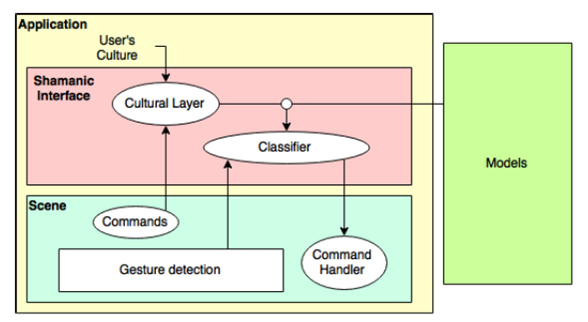
\includegraphics{figures/ShamanicBasicArchitecture.png}
        \caption{\label{fig:ShamanicBasicArchitecture}Basic Architecture of a Shamanic Interface}
    \end{figure}
    
    Previous work defined an application that followed this basic architecture. However, this operation is insufficient for the purposes of the present work’s design. One major change in the requirements is the need for multiple classifiers during completion of the game, hence, the ability for the Shamanic Interface to react to context switching, such that gestures that previously should be recognized as commands no longer should be recognized in the same manner, if at all.\\
    This is where the concept of \emph{State} is introduced. States are a smaller selection of Commands which will generate a different Classifier. Instead of being discarded from memory, the Cultural Layer is always kept in memory, ready to generate new Classifiers on demand. There’s a number of advantages to this approach. Compared to receiving commands but ignoring it at application level, there are benefits to classification accuracy in generating a classifier with only the fewer actions required. This also provides a larger degree of potential adaptability to the interface based on implementation, given that it provides a method by which the application can fall back to alternate classification. With this change, an additional stage of communication is added between the Application and the Shamanic Interface.\\
    
    \begin{figure}[ht]
        \centering
        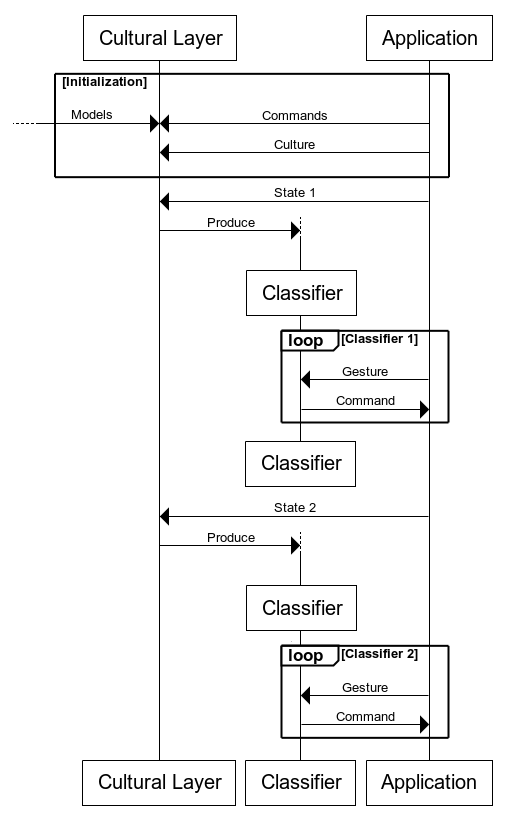
\includegraphics{figures/SequenceDiagram.png}
        \caption{\label{fig:ShamanicSequenceDiagram}Interaction Diagram for generation and usage of multiple Classifiers}
    \end{figure}

\subsection{Gesture Classification and Recording} \label{sec:develop_Classifiers}
    The method used for Gesture Classification is specific to each implementation of a Shamanic Interface. Optimally, classification and type of models used would be an entirely decoupled and independent process so the interface can be more adaptable to new solutions. Nevertheless, given the scope of the present work being very small and, while the Shamanic Interface in its state, given the separation of roles between the cultural layer and the classier, could easily be further refactored to make use of alternate models, the module employed makes use of a single gesture detection method and would require further work to generalize its model usage.\\
       
    %Pagebreak required so the image shows up here instead of several sections later.
    \clearpage
    
    As stated previously in the opening of this chapter, the models used to generate Classifiers with are built using an Accord.NET library's Hiddden Markov Learning module. The Classifier is loaded with gesture classification models based on Hidden Markov Model, in simple terms, state machines where each state has probabilistic transitions. The Classifier acts as a filter, outputting the most likely match between an input noisy set of data values (the recorded gestures) and each of the models. The filter yields matches above a threshold probability, and defaults to the neutral gesture, the first one loaded, if none of the models has a good enough fit. To achieve this setup, it was required to create, and therefore train, these gesture classification models to load the Classifiers with. Thus, the models were trained by employing an unsupervised learning algorithm called the Baum-Welch Learning Algorithm, and utilizing a Forward Topology for the Hidden Markov Models. The number of states permitted in the Model's topology is customizeable before training, with more states often resulting in higher likelihood of accurarcy, but requiring longer amount of times to produce the model. Models were trained with static tolerance, but with different levels of Forward states, starting at 6 and going up to 20, with all but the best matching model discarded and the remaining one then tested and incorporated into the shamanic interface. More information on training these models can be found on \cite{classHMMAlgorithms}.\\

    As for the recording of Gestures to produce the models with, little work was done to the prior Gesture Recorder application beyond compatibility necessary with the Shamanic Interface’s end. Sequences of Gestures are recorded using the same Leap Motion device that will later perform Gesture Detection during the game’s application. These Sequences are captured as Frames, structures detailing hand and finger directions and movement during the recording segment. A total of 200 sequences were recorded for each gesture and each hand, to be used as training data for the models (4000 samples spread accross 20 classes).

\section{Game} \label{sec:develop_game}

    Alluded to above, the application developed and to performed during the user trials is a culturally enriched experience involving hand gestural control. Put another way, the application is a Game, which is how it will be referred to henceforward in this document, and evaluation involves observing users perform its completion.\\
    It’s a first-person perspective game, controlled exclusively by means of hand gestures detected by the Leap Motion Controller. The game runs on the Unity Engine, making use of Leap’s 3.2 SDK to give it the ability to both show the user’s hand within the game world as a virtual representation, and also to obtain all the frame data from its detection. This frame data is then redirected it to the Shamanic Interface’s Classifier, which handles the interpretation of Gestures into commands. The user goals for the game is to explore the environment and finish a number of tasks, which are distributed in a series of rooms. The game is mostly linear, and the controls are very simple, featuring basic forward and back movement, sideways turning and then a number of commands executed by a cultural emblem.\\

    
    \subsection{Tasks Definition and Design} \label{sec:develop_task_definition}
    From the very start, the game was thought of and designed to act as a frontend for the delivery of segregated and quantifiable cultural events. The idea of creating a gameplay loop involving separate \emph{Tasks} predates this work and is a method often employed in user trials involving usability testing. What’s essential about the tasks is it permits highlighting observable and surveyable data within measurable parameters. These include: User Error, Annoyances and frustrations, Speed of Completion, Attitudes of satisfaction, Requests for help among others that may emerge during trial.\\ 
    The tasks are independent from one another, one action can not alter the function of another task, however, each individual task may involve performing at least more than one action given that these follow a natural flow in the view of the user. This independence extends to the task of moving the character. While performing a task, the player is locked in place and may not move until the task is complete, so that the participant isn’t confused or distracted with technical aspects of control besides that which they contextually expected to perform.\\
    The trials have two different user group, as informed previously. One group is given a natural and cultural experience, while the second group is given the same experience without the cultural components. The difference is established in the Task Definition. The first group, denominated the Cultural Group, performs tasks by means of actions corresponding to Emblems for their culture that fit the task’s context. And a minimum amount of attrition is predicted in negative observable parameters for this group. Meanwhile, the other group, the non-Cultural group, performs the same tasks but the corresponding gestures are evocative of the mimicry or the general context the task is inserted in, but is not a culturally validated first choice.\\
    With the validation of three independent helpers of the same Portuguese culture and age as the eventual participants, two sets of tasks and corresponding command hand-gestures was decided upon as detailed on table \ref{tab:Table_Gestures_Game}. All cultural group emblems were previously selected from a list of well-known and widely spread emblems to mid-Western European cultures, and this verification made sure they were recognizable to Portuguese people. Furthermore, tasks were separated into 2 groups, one, tasks T1 through T4, involving mandatory goalposts the user must go through during the trial, and the other, tasks O1 through O4, involving optional tasks they may choose to skip to end the trial earlier.\\
    
    
\begin{table}[ht]
    \hspace*{-1cm} 
    \centering
    \begin{tabular}{|c|c|c|c|}
    \hline
    \rowcolor[HTML]{C0C0C0} 
    Sigle                         & \textbf{Task}               & \textbf{Cultural Group}                                                            & \textbf{Non-Cultural Group}    \\ \hline
                                  & Move Forwards               & \multicolumn{2}{c|}{\begin{tabular}[c]{@{}c@{}}Point Forwards (Index)\end{tabular}}                             \\ \cline{2-4} 
                                  & Move Backwards              & \multicolumn{2}{c|}{\begin{tabular}[c]{@{}c@{}}Point   Backwards (Thumb)\end{tabular}}                            \\ \cline{2-4} 
                                  & Turn Left                   & \multicolumn{2}{c|}{\begin{tabular}[c]{@{}c@{}}Point   Left (Thumb)\end{tabular}}                                 \\ \cline{2-4} 
    \multirow{-4}{*}{\textbf{M1}} & Turn Right                  & \multicolumn{2}{c|}{\begin{tabular}[c]{@{}c@{}}Point   Right (Thumb)\end{tabular}}                                \\ \hline
    \textbf{T1}                   & Call to Come Close          & Closing a hooked Index                                                             & Wave                           \\ \hline
    \textbf{T2}                   & Display Impatience at delay & Look at opposing wrist                                                                            & Open hand forward              \\ \hline
                                  & Call for Help               & Wave / Raise Index                                                                 & Thumbs Up                      \\ \cline{2-4} 
    \multirow{-2}{*}{\textbf{T3}} & Direct Towards Object       & Point At                                                                           & Pointing, Finger gun style     \\ \hline
    \textbf{T4}                   & Celebrate Victory           & Raising Fist Pump                                                                  & Thumbs Up                      \\ \hline
    \textbf{O1}                   & Silence                     & Index Over Lips                                                                    & Thumbs Down                    \\ \hline
    \textbf{O2}                   & Frame Photo of a flower     & \begin{tabular}[c]{@{}c@{}}Square Corners with indexes and\\   thumbs\end{tabular} & Pinching the imaginary flower  \\ \hline
    \textbf{O3}                   & Pick Telephone              & The “Shaka” hand                                                                   & Raise hooked Index upwards \\ \hline
    \textbf{O4}                   & Shoo Away                   & \begin{tabular}[c]{@{}c@{}}Strike air from inwards to\\   outwards\end{tabular}    & Wave                           \\ \hline
    \end{tabular}
    
    \caption{\label{tab:Table_Gestures_Game}List of Gestures performed on each Task by the Cultural and Non-Cultural groups.}
\end{table}

    Within the game, Tasks are performed in isolation from one another, including the movement. There’re two reasons for this separation. Firstly, so that a user is not encumbered by the possibility of issuing the wrong order while attempting to solve a different prompt. This could be the case if movement is available at all times, and a task’s completion was based on proximity to the task’s location. Secondly, so that a user is capable of identifying a prompt in the first place, as opposed to, for example, the possibility of a user attempting to complete a task with a non-interactive part of the environment, expecting it to respond.\\
    However, Tasks are not meant to be separated within the \emph{‘physical’} space of the virtual world. If that were to be the case, then there would be no requirement to have movement as an option, but rather, all tasks could be tested individually one at a time in each of their own virtual spaces. It was, however, considered that the experience would prove to be more immersive and memorable to the users, thus closer to a natural experience, by giving the player the agency and freedom of the movement option between tasks. The opposing solution was compared to a test or a checkmark examination.\\ 
    To ensure that the game offers no confusion in regard to what current task the game is prompting, and where tasks are located, there is a requirement for both visual and interactive feedback from the game. As such, it was necessary that Task transition fit the following criteria:
    
    \begin{itemize}
        \item Clearly identifiable visual labelling of a task’s location and spatial range of its correspondent state transition.
        \item Clearly identifiable differentiation between a completed and an incomplete task.
        \item Clearly identifiable differentiation between a mandatory and optional task.
        \item Clearly identifiable differentiation between each task type.
    \end{itemize}

    The design that fulfils these criteria was that of the Interaction Space, detailed in image \ref{fig:FigureInteractionSpace}. The interaction space is comprised of two main elements. One being a colour filled floor-level ring that signals to the player the radius the task will take place in and its current state. With a mere glance, the players are able to tell what stage of priority a task has towards their progress and if they should approach it or not in regard to that information, fulfilling 3 of the above requirements. The fourth requirement is fulfilled by the other element, which is a collection of surrounding environmental and interactive props that produce light, sound and movement.\\

    \begin{figure}[ht]
        \hspace*{-3cm}                                                           
            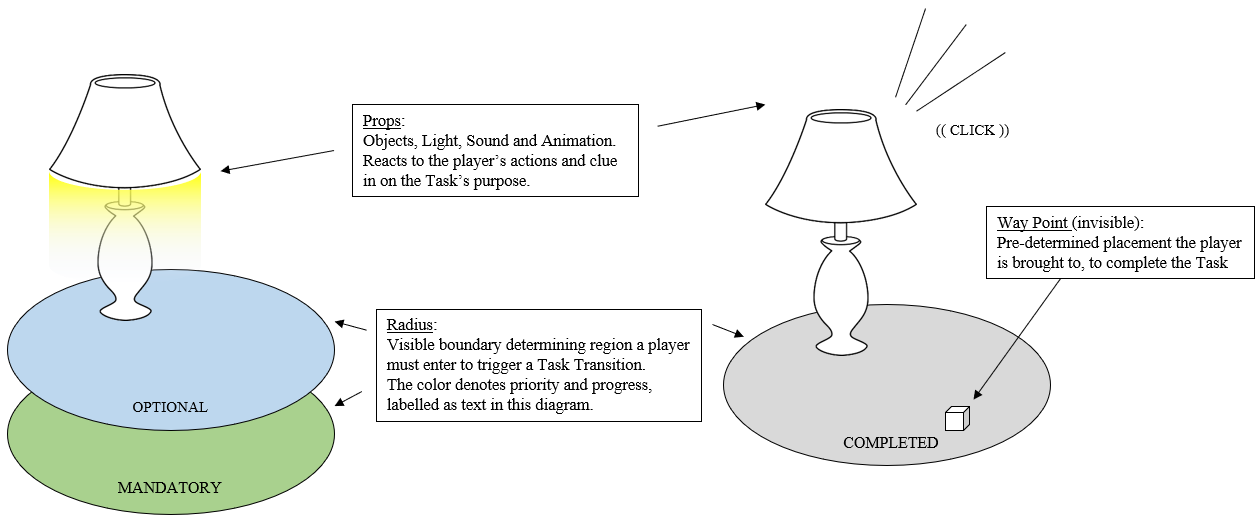
\includegraphics[width=0.95\paperwidth]{figures/InteractionSpaceDesign.png}
            \caption{\label{fig:FigureInteractionSpace}Overview of Interaction Space's Design Elements}               
    \end{figure}
    

\subsection{Player Character Design} \label{sec:develop_character}

    Given that the game was supposed to be a natural and immersive experience, no attention was desired to be brought to a character the user controls. Rather than creating one, the intent was to create an outward sense of belonging into the virtual world, as if the user could say “I am the character on-screen”. Implementing a person even just through aesthetic design could compromise that plan. This was the reason why the game was built with its first-person perspective, that would eliminate the need for any visible character traits on-screen or any latent thought of piloting something over those of self-control.\\
    However, merely showing nothing has one significant issue related to the novelty of the technology used. The Leap Motion is primarily used as an accessory apparatus to Virtual Reality experiences and games, and VR is itself a still uncommonly used technology, with many folks not having first hand experiences with it. The volunteers were predicted to not be completely aware of correct usage or limitations of the device unless if the game provided such feedback live as it occurs, and there isn’t enough time during a user trial to reach the level or proficiency required to innately recognize problems as they arise. A virtual representation of the player’s hand isn’t just a suggestion brought up by other applications of the Leap Motion device, but a requirement that must be present within the game, as then, the user is capable of discerning not just if they’re doing the correct gesture from the representation, but also if the application finds that they’re doing the correct gesture as well, or if small corrections will be required.\\
    Here, a decision is made that is at odds with the problem that caused the choice itself. What should the hand look like? There’re essentially only two possibilities: Either the hand looks realistically, but inevitably appears different from the user’s own real hand and a dissonance is established; or the hand is made to appear like an unambiguously digital approximation of a hand with simpler shapes. There were two at least two hand models provided by the Leap Motion’s library of assets that made either choice possible without much trouble. Given the two choices, no benefit is posed by the first option, and a lesser consistent experience among volunteers was predicted, not to mention the potential source for distraction provided by the more visually enticing.  There was a third option, giving the user a choice of hand model among a larger number, however, that could also pre-emptively give too much of an importance to the hand’s look, which is an undesirable outcome if avoidable. \\
    As such, during the game, the player can see a hand’s model built of simple gray and blue smooth shapes denoting fingers and joints, functioning as a proxy to the player’s own hand, and reacting to movement by performing the same gestures and staying at a similar depth and distance as the player’s own real hand would, mimicking a first person’s field of view with a raised hand.\\

    \begin{figure}[ht]
        \centering                                                
        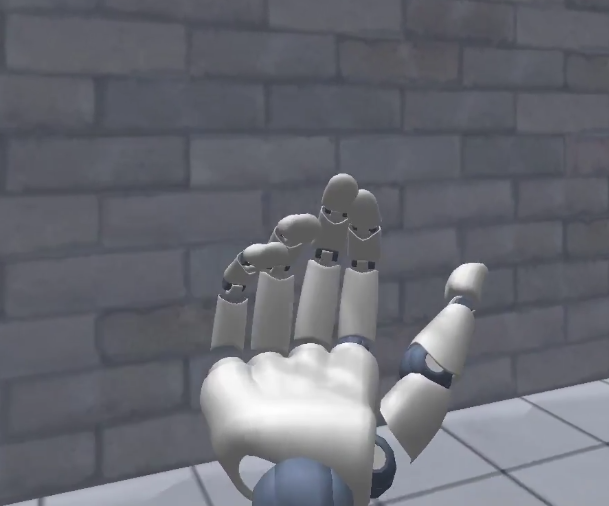
\includegraphics[width=0.3\paperwidth]{figures/HandIngame.png}
        \caption{\label{fig:FigureHand}Screen Capture of the in-game Hand Model}               
    \end{figure}

\subsection{Enviroment Design} \label{sec:develop_game_enviroment}

    The game occurs in a single virtual environment. Once it begins, there are no loading screens and any pauses happen only due to the game’s own interactive make up rather than to needing to load more assets. The only complex background processing required involves the classifier switching and even this should be a seamless and instant process. In other words, the game is small enough to be fully loaded at all times.
    Yet, it should also have been big enough that there isn’t a perception overload to the player with too many tasks and options present at a time. A large multiplicity of cues can confuse or frustrate the user. Given that there are 8 total tasks in the game separated in two groups of four, it was found appropriate to separate these into pairs of two tasks, one mandatory and one optional, and placed within four rooms. Additionally, to streamline the process of finding these tasks, the rooms were laid out in sequence through connecting corridors.\\
    
    \begin{figure}[ht]
        \centering
        \hspace*{-1cm}
        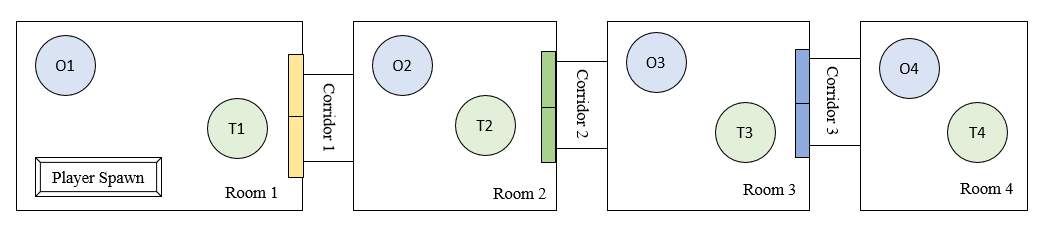
\includegraphics[width=0.8\paperwidth]{figures/RoomOverview.png}
        \caption{\label{fig:FigureRooms}Overview of the virtual enviroment's Room Design}
    \end{figure}

    One of the things that such a sequential line-up opens to the game is the chance of someone missing out on the presence of a task. This is undesirable, as detracting user choice from the completion of a task gives off less information about the task itself, than someone intentionally avoiding it or performing it and giving a bad grade. Opposed, to it, it does permit to observe one of the subtler factors of immersive experiences, assumingly, the user’s level of comfort and confidence with the controls, which are often overstated in self-assessments. Ultimately, the proposition of an intuitive cue for progress trumps over alternatives.\\
    Rooms are therefore separated by gates that do not open until the containing mandatory task is finished. Moreover, the transition between rooms is not just identified by the crossing of a gate, but also visually by the rooms themselves, as the looks of the floor, walls and ceilings changes drastically upon entering a corridor and matches with the following area. Also, to better attach the completion of a mandatory task with its correspondent gate, these gates were colored, and a key was integrated as part of the task’s completion.\\
    Other guiding elements are also present within rooms. Green arrows appear near gates, corridor entrances or on empty walls to help direct the user and reinforce that they’re heading the correct direction. Non-interactive plants are present on empty corner to fill the empty space and give the impression of a location of no interest to the game’s progress. Also, the empty play area with no object of interest is progressively funnelled in size, as the player is expected to make lesser mistakes in their movement as they progress and would find less of a reason to take large exploratory measures with the controls.\\ 
    This last point touches on the subject of room layout, which brings up the question of task placement. Of the two tasks in each room, the mandatory task is always placed closest to the exit gate and furthest to the entrance. The optional tasks however are progressively brought into the most direct path of the player. In order: O1 is on an indentation to the left of the room, O2 is off to the left but within the regular room boundaries, O3 is to the left of the path, but directly in front of the player from where they would come into the room, and finally, O4 is completely in the way of the player and they must sidestep it if they don’t want to compete the task. Additionally, O1 and O2 represent tasks that don’t lend themselves to having very much of an immediate urgency in nature, while O3 and O4 represent something that demands hurriedness from the user, and something that is just bothersome and has to be dealt with right away, thus justifying their progressive shift from staying away to getting in the way.\\
    
    \begin{figure}[ht]
        \centering
        \hspace*{-1cm}
        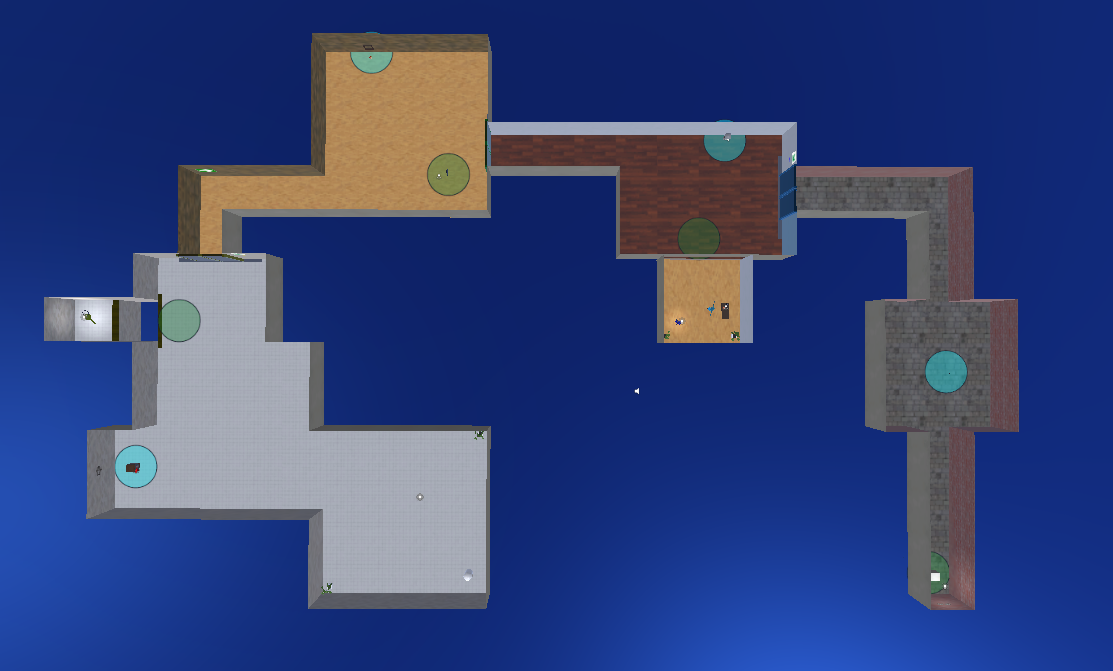
\includegraphics[width=0.8\paperwidth]{figures/Overhead.png}
        \caption{\label{fig:FigureGameOverhead}Overhead view of the game's virtual enviroment}
    \end{figure}

\subsection{Game Logic} \label{sec:develop_game_logic}
    For its implementation on Unity, the game has 4 core elements. These are the \emph{GameController}, \emph{CharacterController}, \emph{InteractionSpaceController} and \emph{CinematicHandler} scripts. Many other scripts were relevant to the game’s function, however, all of those had a small role within restrained contexts, and worked in a master, slave manner to one of these core scripts, such as, for example, the RadomFlight handler script, that made task O4’s insects move erratically, does not interact with any script besides the CinematicHandler and does so only on one moment in the game, during the closing transition of the O4 interaction space.\\
    The \emph{GameController} is tasked with initializing the game’s Shamanic Interface and defining state definitions that the game will require. It is also the game controller that will dispense a new classifier during task transitions. Thus, this Is an entry point for the Character Controller and the Interaction Space Controller during those times. It is also the GameController that defines the game’s culture, and it is here that I found the single difference between the game build presented to the Cultural and Non-Cultural groups. The Non-cultural group plays with an undefined Culture and thus the game uses the SI’s default gestures. Meanwhile, the Cultural group defines its culture as “PT” and those gestures get overridden by the pairs belonging to it. The code snippet corresponding to gesture efinition can be found on appendix \ref{ap1:InitCulturalLayer}. There’s a single Game Controller object in the game space and the other core scripts have a reference and access to it at any given moment.\\
    The Character Controller is a long script with definitions related to accepting input from the Leap Motion device (or Keyboard, for debugging purposes) to move the player’s camera around the virtual environment or to complete tasks. It’s here that the game checks if the classifier yields the correct gesture and if it’s also here that the game informs the rest of the system what gesture is currently being performed. It’s also where the game’s current valid options for control are changed, and where collision between a player and an interaction space’s region is handled. Ironically, the Character Controller is not statically aware of any command definition, merely matching what the classifier informs it, with the current Task. Its task completion code being agnostic to the definitions allows it to function if new definitions are set up. In summation, anything related to player input or to changing what a player can do has its entry point here.\\ 
    However, it’s the Interaction Space Controller that defines what those gestures are for each task, and if they’ve been performed for long enough to accrue to the task’s completion. While there is a single Character Controller there’s a different instance of the Interaction Space Controller attached to the corresponding game objects. Every interaction space object has its own script, with its own different internal settings correspondent to a different Task. Upon collision of the Player and an Interaction Script, the scripts belonging to each attach to each other, and a back process of communication ensues through the 3 Scripts. The Interaction Space controller informs the Character Controller of what Task is performed within the interaction space, and the Character Controller then requests the Game Controller To feed that task’s correspondent State into its Shamanic Interface. Finally, the Game Controller yields the resulting Classifier back to the Character Controller, and the Character Controller will from then on inform the Interaction Space every frame that a gesture was performed. State definition code snippets can be found in \ref{ap1:StateDefinitions}.\\
    This happens relatively instantaneously, albeit, there is some leeway to give the Shamanic Interface some time for returning the Classifier, as at the very first moment of the collision between player and Interaction Space, an initial task transition phase, called player repositioning, is executed. During these, the character controller actually removes control from the player for three seconds and forcefully moves them to an appropriate spot where they will perform the task’s gestures.\\
    And, finally, the Cinematic Handler, which synchs and performs visual and audible alterations to the environment during intermediate and final task transition phases. From moving and animating object, to dimming lights and turning off sounds, this provide the player with the feedback that a Task was completed by changing the task’s props in some manner. Only the Interaction Space Controller communicates with it, which means that granting player control after a Task’s completion must be done through it as a middleman between the Cinematic Handler and the Character Control Script.\\

    \begin{figure}[ht]
        \centering
        \hspace*{-1cm}
        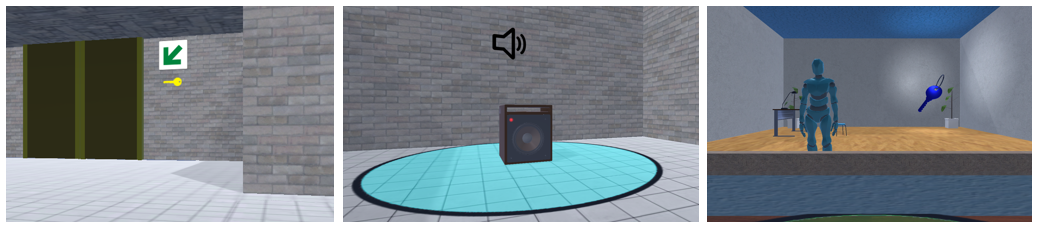
\includegraphics[width=0.8\paperwidth]{figures/IngameScreenshots.png}
        \caption{\label{fig:FigureScreenshots}Screenshots of the Game Enviroment}
    \end{figure}
\section{Volunteer Trials} \label{sec:develop_trials}
    This works’ field research is composed of, as determined before, user trials in a controlled environment with the goal of finding and collecting insight in regard to the usage of Cultural Awareness as the primary solution for the issue of user spontaneity and adaptability, and the hypotheses stated within the Goals section\ref{sec:intro_goals}.\\
    The planning surrounding the user trials was carried out with the intent of facilitating the forms of techniques employed in data collection useful for evaluation, those being observation data and user opinion data. These are performed concurrently to differing degrees of focus in accordance to different parts of each trial. These parts of a trial roughly follow the directions of the outline provided earlier in the section on HCI Evaluation\ref{sec:hci_definition_goals}, however, they will be detailed further in the following sections and an overview provided is provided in image \ref{fig:FigureTrialSections}.
    
    \begin{figure}[ht]
        \hspace*{-1cm}
        \centering                                                
        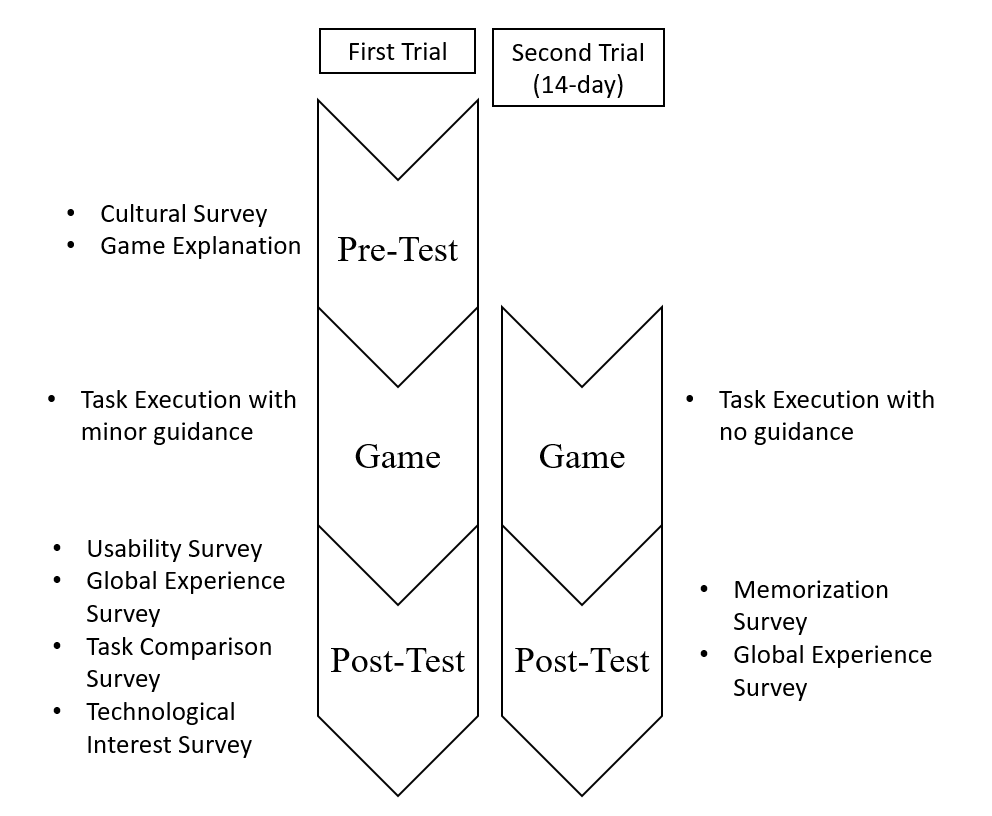
\includegraphics[width=.9\paperwidth]{figures/TrialSections.png}
        \caption{\label{fig:FigureTrialSections}Overview of User Trial's Sections.}               
    \end{figure}
    
    \subsection{Pre-Test} \label{sec:develop_trials_pre}
    The pre-test is the initial part of the trial, and it matches up roughly to the Introduction and Warm-Up phases of a field study plan. Users are introduced to the controlled environments, the room and equipment, and are initially asked for their demographic data and some first impressions and some very basic questions, such as, if they have knowledge of the apparatus used in gesture detection presented, the Leap Motion. They are also allowed to test out the Leap Motion’s diagnostic visualizer for up to 30 seconds just to get a rough idea of its function.\\
    However, there’s two bigger main components to the Pre-test after the initial introduction. A Cultural Survey and a Game Explanation.\\
    The Cultural Survey is done before any information about the game is given to the volunteer. They are presented with a simple black text on white background slide show containing several snippets indicating a different message. Each message represents one of the game’s task, and the volunteer is tasked with performing the gestures they feel best describe that action or message. The main objective of this exercise is checking if the user performs a majority of the same moves as the ones the Cultural Group uses during the game. This is a requirement of this work as a counter-measure against certain potentially erroneous assumptions made during development, such as, most directly, the choice of gestures the tasks use. Should the majority of users name the same gestures as the Cultural Group, this helps pre-emptively validate the game as a cultural experience. Should the majority name a specific different gesture, that should, conversely, invalidate that task for result-checking.\\
    The Game Explanation happens right afterwards. Here, the volunteers are shown a depiction of the in-game tasks they’ll have to perform, in the same order as the messages they just read through, both in the slide show and with a separate physical document. There are different explanations for the cultural and non-cultural group, however, those difference are never stated. The volunteers are given instructions on how to perform the tasks, as well as the differences between the Interaction Spaces and the method by which the game progresses. Finally, they’re asked if they understand the purpose of the gesture used in the task. Their comments and understanding are written down and recorded. Here the non-cultural users are implicitly given an opportunity to name their preference for one of the tasks they performed previously.\\
  
    \subsection{Game Observation} \label{sec:develop_trials_game}
    Following the explanation of the game, the volunteers are ready to play the game proper. Here, they are asked to perform the game fully. The volunteers are given a few more pointers to aid them on the way, mainly with getting used with movement, but are never outright given the actual gestures required for a task. They are also prompted for help if they appear to have difficulties at certain steps but are only given it if they accept or request it.\\
    Any special observation is recorded, priority given to unexpected displays of frustration or amusement. But some aspects of observing the user are most important for this segment. The Time Elapsed, the Number of User Errors, if Help was Required, and if the Correct Gesture was actually performed. These are likely to provide the most qualitative insight and are discernible enough to make an immersion scoring out of, and as such, the protocol developed for the trial is to document these values for every single task and every single volunteer, with both help from recordings (when permitted) and the game’s own logging of each task.\\

    \subsection{Post-Test} \label{sec:develop_trials_post}
    After the game is completed, the volunteer is given a moment to rest and then they’re asked to go over a questionnaire and answer it. This is closely related to the Cool-Off period of a field research and is the adequate time to investigate questions in the form of a survey. Volunteers aren’t asked to answer on their own, but rather, all of the questions are read out to the users and they’re made clearly aware of what each question is asking, slowing down the pace between questions if they’re answering too fast, and prodding for certainties in responses when a bout of indecision arises.\\
    There are three parts to the post-test questionnaire. The first part is a usability survey. Since the game was rewritten from scratch, it stands that its usability is still unproven and must be evaluated, however, the real reasoning behind making this investigation is that many aspects of usability have crossover with immersion and satisfaction signifiers. Thus, this is an insightful exercise towards the goals of this work and helps frame the way by which further questioning will be administered. The questions presented in the first part are adapted from the System Usability Scale. All scores of the scale are present and answers are scaled such as a 0-100 usability score is possible. Some other satisfaction-related questions were dropped here, particularly, that of the least enjoyable or most concerning aspect of the game, to ensure users don’t leave out details about their frustrations.\\ 
    The second part of the questionnaire goes over every Task and asks two questions on a scale for each of the gestures. The two aspects are surveyed are the ease of the gesture, and the natural fit of the gesture for the task. Since the users may find different interpretations for the scale, this one is meant to be taken as a comparative measure between each of the gestures, scoring them in terms of ‘below than ideal’. This should provide some final insights into the choice of gestures and their applicability for the task, but moreover, should provide a focal point of comparison between the Cultural and Non-Cultural groups.\\
    The third part is short, and merely looks into the volunteer’s experience with computers on their daily lives and their interest and pre-existing capabilities using other natural systems. This was a concern that could arise if groups of volunteers appeared to have vastly different expectations and performances between one another.\\
    
    \subsection{Second Trial} \label{sec:develop_trials_second}
    After performing the trial, the users are thanked and allowed to depart. However, their contribution isn’t over at this point. Given that one aspect of the proposed benefits to the shamanic interface approach has a large emphasis on memorization of commands, these have to be tested after a delay of time with no exposure to the system. All participants are therefore asked to come back and fulfil a second follow-up trial after a period of 14 days minimum. The goal here is to assess if their memory of the content still matches the actual experience. The second trial has two parts, first the volunteers perform the game again, and then they’re given a new post-game questionnaire.\\
    Absolutely nothing is changed with the game builds themselves, as the experience must remain consistent with the previous. Also, the same indicators have primary focus during observation, those being Number of User Error and so on. However, a small difference is with the protocol is that time, the users are not given any of the previous helpful pointers and are not prompted on their need of help if they’re seen struggling. The players must request help themselves if they appear to struggle and are allowed to proceed with failure if they don’t remember the task gesture but are certain of an erroneous one. This compels users to rely only on their own recollection of the solutions and in taking their time, rather than rely on communication with the researcher. The benefit of taking this approach is that it highlights their confidence on the gestures given without it needing to be taken in survey. To that end, the users are also not corrected on gestures until the second trial is over and they’re no longer under observation.\\
    The second post-game questionnaire is different from the first trials. This questionnaire has two parts. The first goes over every task and surveys users on their ease remembering each gesture. This is, again, meant to highlight a difference between each of the two Cultural groups, as the Non-cultural is predicted to mention greater barrier against the Cultural group. Additionally, there may also be a significant disparity between self-confidence and erroneous resolution of gestures in this aspect between the two groups, which may be of interest to record. As for the second part of the questionnaire, instead of focusing mostly on usability like the previous, this time, users are prompted over categories of experiential quality indicators. They’re asked about the impact, agreement and value of several aspects of the experience which they may rate on a 5-point scale between Strong Disagreement and Strong Agreement, although the majority just kept to simple a binary dimension between Yes and No or Good and Not Good answers. Listing the categories, their affective expectations, their feelings, their self-consciousness, the repeatability and their willingness to share with and recommend to others, their thoughts on the applicability and usability of the type of experience among different groups of people, the technological quality of the experience, and sense making and meaningful feedback.\\
\chapter{Results} \label{chap:results}
%\section*{} \label{sec:...}
%\begin{dummied}
%\end{dummied}

    The user trials were conducted at the Faculty of Engineering from University of Porto within labs and other rooms, in isolation from each other and from the presence of distracting elements such as other people not part of the test. Excluding a user requested to conduct a pilot trial ahead of the remainder, from a much larger pool of signed up people a total of 17 users performed the trials, 16 of which saw the second trial to completion. The research observer for the trials was the author of this document, who sat beside the volunteer at a table with all the equipment and required paper files. User sessions have been recorded with given explicit consent.\\
    Results, observations and analysis of the data will be given in this paragraph. The impact this analysis had on the hyposteses will be laid out in sumation on the Conclusions Section \ref{sec:results_Conclusions}.

\section{User Sample Description} \label{sec:results_section}
    As remarked above, the trials involved 17 participants, from whom 16 have concluded the whole two phases of trial and one has failed to attend the second trial. The participants were divided in two groups, the cultural group with 9 participants, and the non-cultural group. Given that participant number 5, the person who did not have the availability to show up to the follow-up trial, belonged to the Cultural Group, this leaves the results with 17 cultural evaluations during the pre-test, and then a balanced 8 evaluations for the Cultural Groups and 8 evaluations for the Non-Cultural Group.\\
    The participants were all portuguese students from University of Porto, belonging to different faculties and courses, although the majority reports studying a field of engineering. As such, the age gap is constrained to the 18-24 gap, and demonstrate at least some domain knowledge in technology, even if none showcases any experience with the equipment. Still, two particular users, number 1 and number 8, stood out from the remaining where Technological and Domain Interest was looked at, to which both have been further questioned and both have answered to currently work in the field of study of Informatics.\\
    The sorting of volunteers between Cultural and Non-Cultural groups was done in the most randomly and balanced approach available, while weighting the possibility of volunteer drop-out. The first user was tested and observed within the Cultural Group and then each participant was interleaved to the Non-Cultural Group and the Cultural once again in accordance to their scheduling order, which is equivalent to their participant numbering. As such all odd-numbered participants would belong to the Cultural Group and all even ones would belong to the non-Cultural. However, a slight alteration was found necessary, by questioning the users early on if they knew someone else who would also participate in these trials. Two volunteers claimed to know each other, number 4 and number 7, and as such, participant 6 was slated to belong to the Cultural Group ahead of time so that 4 and 7 could both belong to the same group. This such change as to not have them influence each other’s memories with erroneous impressions of the other’s trials by sharing them between each other. Sharing impressions of the first experience with other people was not forbidden and is actually encouraged as one of the potential immersivity signifiers, however there may be a potential unexpected effect from the sharing of mismatching experiences that was thought best avoided. By giving them both the same experience, they could instead only reinforce or re-consider aspects they have witnessed first-hand and make their own impressions for the second experience survey.\\
    Table \ref{tab:Table_UserDemographics} lists user demographics as well as findings on the user’s technological interests.\\

    % Please add the following required packages to your document preamble:
    % \usepackage{multirow}
    \begin{table}[ht]
    \begin{tabular}{|l|l|l|l|l|l|}
    \hline
    Volunteer Number & Gender & Main Hand & Age & Tecnological Interest & \multicolumn{1}{c|}{Group}    \\ \hline
    1                & M      & R         & 23  & 9                     & \multirow{9}{*}{Cultural}     \\ \cline{1-5}
    3                & M      & R         & 21  & 7                     &                               \\ \cline{1-5}
    5                & M      & R         & 21  & 8                     &                               \\ \cline{1-5}
    6                & F      & R         & 22  & 4                     &                               \\ \cline{1-5}
    9                & M      & R         & 24  & 5                     &                               \\ \cline{1-5}
    11               & M      & R         & 23  & 6                     &                               \\ \cline{1-5}
    13               & M      & R         & 21  & 3                     &                               \\ \cline{1-5}
    15               & F      & R         & 18  & 8                     &                               \\ \cline{1-5}
    17               & F      & R         & 22  & 7                     &                               \\ \hline
    2                & F      & R         & 18  & 6                     & \multirow{8}{*}{Non-Cultural} \\ \cline{1-5}
    4                & M      & R         & 23  & 8                     &                               \\ \cline{1-5}
    7                & M      & R         & 19  & 7                     &                               \\ \cline{1-5}
    8                & M      & R         & 21  & 10                    &                               \\ \cline{1-5}
    10               & F      & R         & 24  & 7                     &                               \\ \cline{1-5}
    12               & M      & L         & 23  & 7                     &                               \\ \cline{1-5}
    14               & M      & R         & 22  & 6                     &                               \\ \cline{1-5}
    16               & M      & R         & 23  & 7                     &                               \\ \hline
    \end{tabular}
    \caption{\label{tab:Table_UserDemographics}Listing of Volunteer Demographics Findings and Sorting within Cultural and Non-Cultural Groups.}
    \end{table}
\section{Cultural Experience Validation} \label{sec:results_culturalvalidation}
    The pre-test was a common section that all 17 volunteers performed, still unaware of the User Trial’s goals or even general setup beyond the knowledge that cultural gestures would be an essential part of the observation. With no pre-emptive knowledge of the experience and with, at this point, very little suggestive information as to what will be required of them, they were surveyed, using simple language and a simple presentation, on what they found was the correct set of emblematic gestures that would solve or address each of the specific Tasks they would later have to employ in the game. Before beginning, the users were assured that no such thing as a wrong answer could possibly exist as this was a direct survey of their personal opinions, and they were put at ease that none of the data lifted would result into later questioning, as this data would have no relation with the experiment ahead.\\
    Ideally, this would be performed on a different set of users beforehand, which would even allow for a restructuring of the methodology employed on the user trials as a whole, exploring aspects such as natural discovery of commands without guidance. However, given the limited availability of volunteers and the likelihood of dropout in a two-part experiment, it was found hard to do so within the means reachable.\\
    If a Task’s chosen gesture is correctly selected and fit for the purposes of a Cultural Experience, then when given the opportunity to perform the Task on any independent context, a person should most of the time opt to perform that same well-fit gesture over another. Admittedly, certain scenarios may change the chosen gesture due to certain contextual cues lending towards different interpretations, and on top of that, not all gestures that abide by this are necessarily emblematic. For example, working with certain tools may represented by an emblematic gesture, by limiting the shape of the tool to a different arrangement may lead the person to perform a less emblematic gesture, and instead perform mimicry of the action. This concern was actually predicated in the design of the game by the optional Task O3, answering a phone, which demanded the choice on in-game representation of the ringing Phone be an object with a handset piece that can be held, as opposed, for example, a more modern looking device. This is why in the pre-test, not just were users asked to perform the gesture they find correct without a particular context in the barebones slideshow, but they were also asked if the game’s taught gesture made sense for the context.\\

\subsection{Invalidated Tasks} \label{sec:results_invalid_tasks}
    Table \ref{tab:Table_GestureValidationPretest} is the result of the first part of the pre-test, where all of the volunteers were asked about performing the chosen gesture.

    \begin{table}[ht]
    \begin{tabular}{|l|l|l|l|l|l|l|l|l|l|}
    \hline
    \cellcolor[HTML]{FFFFFF} & O1                        & T1                        & O2                        & T2                        & O3                        & T3.1                      & T3.2                      & O4                        & T4                        \\ \hline
    V1                       & \cellcolor[HTML]{D6FDD5}Y & \cellcolor[HTML]{D6FDD5}Y & \cellcolor[HTML]{FFE7E6}N & \cellcolor[HTML]{FFE7E6}N & \cellcolor[HTML]{D6FDD5}Y & \cellcolor[HTML]{FFE7E6}N & \cellcolor[HTML]{D6FDD5}Y & \cellcolor[HTML]{D6FDD5}Y & \cellcolor[HTML]{D6FDD5}Y \\ \hline
    V2                       & \cellcolor[HTML]{D6FDD5}Y & \cellcolor[HTML]{D6FDD5}Y & \cellcolor[HTML]{FFE7E6}N & \cellcolor[HTML]{D6FDD5}Y & \cellcolor[HTML]{D6FDD5}Y & \cellcolor[HTML]{D6FDD5}Y & \cellcolor[HTML]{D6FDD5}Y & \cellcolor[HTML]{D6FDD5}Y & \cellcolor[HTML]{D6FDD5}Y \\ \hline
    V3                       & \cellcolor[HTML]{D6FDD5}Y & \cellcolor[HTML]{D6FDD5}Y & \cellcolor[HTML]{D6FDD5}Y & \cellcolor[HTML]{FFE7E6}N & \cellcolor[HTML]{D6FDD5}Y & \cellcolor[HTML]{D6FDD5}Y & \cellcolor[HTML]{D6FDD5}Y & \cellcolor[HTML]{D6FDD5}Y & \cellcolor[HTML]{FFE7E6}N \\ \hline
    V4                       & \cellcolor[HTML]{FFE7E6}N & \cellcolor[HTML]{D6FDD5}Y & \cellcolor[HTML]{FFE7E6}N & \cellcolor[HTML]{D6FDD5}Y & \cellcolor[HTML]{D6FDD5}Y & \cellcolor[HTML]{D6FDD5}Y & \cellcolor[HTML]{D6FDD5}Y & \cellcolor[HTML]{D6FDD5}Y & \cellcolor[HTML]{D6FDD5}Y \\ \hline
    V5                       & \cellcolor[HTML]{D6FDD5}Y & \cellcolor[HTML]{D6FDD5}Y & \cellcolor[HTML]{FFE7E6}N & \cellcolor[HTML]{D6FDD5}Y & \cellcolor[HTML]{D6FDD5}Y & \cellcolor[HTML]{D6FDD5}Y & \cellcolor[HTML]{D6FDD5}Y & \cellcolor[HTML]{D6FDD5}Y & \cellcolor[HTML]{D6FDD5}Y \\ \hline
    V6                       & \cellcolor[HTML]{D6FDD5}Y & \cellcolor[HTML]{D6FDD5}Y & \cellcolor[HTML]{FFE7E6}N & \cellcolor[HTML]{FFE7E6}N & \cellcolor[HTML]{D6FDD5}Y & \cellcolor[HTML]{FFE7E6}N & \cellcolor[HTML]{D6FDD5}Y & \cellcolor[HTML]{D6FDD5}Y & \cellcolor[HTML]{D6FDD5}Y \\ \hline
    V7                       & \cellcolor[HTML]{FFE7E6}N & \cellcolor[HTML]{D6FDD5}Y & \cellcolor[HTML]{FFE7E6}N & \cellcolor[HTML]{FFE7E6}N & \cellcolor[HTML]{D6FDD5}Y & \cellcolor[HTML]{D6FDD5}Y & \cellcolor[HTML]{D6FDD5}Y & \cellcolor[HTML]{D6FDD5}Y & \cellcolor[HTML]{D6FDD5}Y \\ \hline
    V8                       & \cellcolor[HTML]{D6FDD5}Y & \cellcolor[HTML]{D6FDD5}Y & \cellcolor[HTML]{FFE7E6}N & \cellcolor[HTML]{FFE7E6}N & \cellcolor[HTML]{D6FDD5}Y & \cellcolor[HTML]{D6FDD5}Y & \cellcolor[HTML]{D6FDD5}Y & \cellcolor[HTML]{D6FDD5}Y & \cellcolor[HTML]{D6FDD5}Y \\ \hline
    V9                       & \cellcolor[HTML]{D6FDD5}Y & \cellcolor[HTML]{D6FDD5}Y & \cellcolor[HTML]{FFE7E6}N & \cellcolor[HTML]{FFE7E6}N & \cellcolor[HTML]{D6FDD5}Y & \cellcolor[HTML]{FFE7E6}N & \cellcolor[HTML]{D6FDD5}Y & \cellcolor[HTML]{D6FDD5}Y & \cellcolor[HTML]{D6FDD5}Y \\ \hline
    V10                      & \cellcolor[HTML]{D6FDD5}Y & \cellcolor[HTML]{D6FDD5}Y & \cellcolor[HTML]{FFE7E6}N & \cellcolor[HTML]{FFE7E6}N & \cellcolor[HTML]{D6FDD5}Y & \cellcolor[HTML]{FFE7E6}N & \cellcolor[HTML]{D6FDD5}Y & \cellcolor[HTML]{D6FDD5}Y & \cellcolor[HTML]{D6FDD5}Y \\ \hline
    V11                      & \cellcolor[HTML]{D6FDD5}Y & \cellcolor[HTML]{D6FDD5}Y & \cellcolor[HTML]{FFE7E6}N & \cellcolor[HTML]{FFE7E6}N & \cellcolor[HTML]{D6FDD5}Y & \cellcolor[HTML]{D6FDD5}Y & \cellcolor[HTML]{D6FDD5}Y & \cellcolor[HTML]{D6FDD5}Y & \cellcolor[HTML]{D6FDD5}Y \\ \hline
    V12                      & \cellcolor[HTML]{D6FDD5}Y & \cellcolor[HTML]{D6FDD5}Y & \cellcolor[HTML]{FFE7E6}N & \cellcolor[HTML]{FFE7E6}N & \cellcolor[HTML]{D6FDD5}Y & \cellcolor[HTML]{FFE7E6}N & \cellcolor[HTML]{D6FDD5}Y & \cellcolor[HTML]{D6FDD5}Y & \cellcolor[HTML]{D6FDD5}Y \\ \hline
    V13                      & \cellcolor[HTML]{D6FDD5}Y & \cellcolor[HTML]{D6FDD5}Y & \cellcolor[HTML]{FFE7E6}N & \cellcolor[HTML]{FFE7E6}N & \cellcolor[HTML]{D6FDD5}Y & \cellcolor[HTML]{D6FDD5}Y & \cellcolor[HTML]{D6FDD5}Y & \cellcolor[HTML]{FFE7E6}N & \cellcolor[HTML]{D6FDD5}Y \\ \hline
    V14                      & \cellcolor[HTML]{D6FDD5}Y & \cellcolor[HTML]{D6FDD5}Y & \cellcolor[HTML]{FFE7E6}N & \cellcolor[HTML]{FFE7E6}N & \cellcolor[HTML]{D6FDD5}Y & \cellcolor[HTML]{D6FDD5}Y & \cellcolor[HTML]{D6FDD5}Y & \cellcolor[HTML]{D6FDD5}Y & \cellcolor[HTML]{D6FDD5}Y \\ \hline
    V15                      & \cellcolor[HTML]{D6FDD5}Y & \cellcolor[HTML]{D6FDD5}Y & \cellcolor[HTML]{FFE7E6}N & \cellcolor[HTML]{FFE7E6}N & \cellcolor[HTML]{FFE7E6}N & \cellcolor[HTML]{FFE7E6}N & \cellcolor[HTML]{D6FDD5}Y & \cellcolor[HTML]{D6FDD5}Y & \cellcolor[HTML]{D6FDD5}Y \\ \hline
    V16                      & \cellcolor[HTML]{D6FDD5}Y & \cellcolor[HTML]{D6FDD5}Y & \cellcolor[HTML]{FFE7E6}N & \cellcolor[HTML]{FFE7E6}N & \cellcolor[HTML]{D6FDD5}Y & \cellcolor[HTML]{D6FDD5}Y & \cellcolor[HTML]{D6FDD5}Y & \cellcolor[HTML]{D6FDD5}Y & \cellcolor[HTML]{D6FDD5}Y \\ \hline
    V17                      & \cellcolor[HTML]{D6FDD5}Y & \cellcolor[HTML]{D6FDD5}Y & \cellcolor[HTML]{FFE7E6}N & \cellcolor[HTML]{FFE7E6}N & \cellcolor[HTML]{D6FDD5}Y & \cellcolor[HTML]{D6FDD5}Y & \cellcolor[HTML]{D6FDD5}Y & \cellcolor[HTML]{D6FDD5}Y & \cellcolor[HTML]{FFE7E6}N \\ \hline
    \end{tabular}
    \caption{\label{tab:Table_GestureValidationPretest}User-oriented Validation of Task gesture choice by mean of blind survey of natural cultural emblems.}
    \end{table}
    
    Two tasks with concerning response arise in a suspiciously distinct manner. Of the one or two gestures each user made for the slide correspondent to Task O2 and Task T2, only very few actually performed the expected Gesture during the Cultural Validation. This punctuates the possibility of having made the wrong assumption for each of the two during the initial brainstorming or subsequent steps involved in this selection of Gestures. Alternatively, it could also signify that the presentation itself was misleading or not clear enough.\\
    To that end, all the diverging answers provided by the users were recorded, in an attempt to figure out if there’s a consistent pattern as to what went wrong in the design of the Task.\\
    Task O2 involves taking a snapshot of a flower and framing it in an initially empty rectangular mount. Already, with care, from this Task description could the problem be perceived, as well as the eventual source of the disparity. The Task describes two actions, the photograph snapping, and framing of the revealed photo. While in design, the action focused upon was the framing action, most users instead focused on the photographic action itself, which involved a mimicry of the snapshot acting. Out of all 16 users that performed a different action, every single one was recorded performing a gesture called the \emph{“Camera Click”}. This gesture was not found as a symbolic emblem while first researching and planning for this work, which was partially the reason that led to the wrong assumption that it wouldn’t be the most natural response to the task’s proceedings. There was some worry about this Task towards the impact it may have had on the global experience, however this worry was put at ease with the second component of this pre-test, as can be seen on table \ref{tab:Table_GestureVerification}, every user in the cultural group stated that the \emph{Framing} emblem was recognizable and fit the game’s context. Every user, but one, Volunteer number 11, who left the comment “Knows the gesture, but wouldn’t see the connection without an explanation”.\\
    Task T2 is a slightly more complicated matter. The task features a large clock and a waiting sign room, and the users are meant to emote their impatience at a long wait. Only three people gave the expected gesture of looking at or tapping the opposite wrist, however, when looking over the other given gestures, no pattern was recognized. A group of three volunteers performed another well fit gesture of bringing their hand to the side of their head, while two volunteers crossed their arms and tried appearing displeased, a gesture that doesn’t involve detectable hand movements. The remaining gestures were singleton examples of emblems corresponding to hurrying other people, threats and then other non-emblematic gestures of disconcerting reasoning. Unlike with the O2 task, were all users performed one, this makes a total of only 7 users performing an adequate emblematic gesture for the given scenario in T2, and 5 users performing non-emblematic gestures. This is an indication that the scenario chosen for task T2 may have not been an apt one for this game.\\
    As such, the data collected for these two tasks is ignored while doing a discrete assessment of the Tasks, since it can’t be fully justified that differences found between the groups are due to the cultural differences of the experience. These, however, still take a part of the global assessment of the experience, as table \ref{tab:Table_GestureVerification} does provide verification that the users understand and recognize that the choice of gesture is fit to both Tasks, even if not their first choice.\\



\subsection{Preeminent Non-Cultural Misfits} \label{sec:results_pretest_noncultural}
    Past the Cultural Validation, volunteers were taught the game’s intended gestures and asked to comment on them, particularly by request of mentioning if they had prior knowledge of the emblem required and if they found it fitting to the Task shown. Table \ref{tab:Table_GestureVerification} is the result of this request. As is evident, the Cultural group almost completely shown agreement with the choice of gesture. This is was an expected outcome.\\
    But for the Non-Cultural Group, the intent was never to obtain an acquiescent response, but rather a mixture. The objective of the gesture selection for the Non-Cultural Group was to avoid the natural choice, but still pick something that could make sense given an alternate context of the task. For example, the task O1, silencing an object, is performed by showing a thumbs down gesture of disapproval at the speaker prop. The contrast between what’s asked and what gesture is required at play here is that, while the thumbs down is an emblematic gesture for the volunteers and could be used in a different scenario where the objective is communicating the request of lowering of a music’s volume, this is not very sensical if the recipient of the gesture isn’t a person. Ideally, all tasks would have a balanced mixture of volunteers finding the gesture fitting and unfitting, but some gestures have got an overtly positive or overtly negative response.\\
    The Non-Cultural Group participants seemed to focus most on the negative at this step, which is why the presence of task O2 as a major negative read is preeminent. For the positively approached gestures, a difference between the response and the actual performance in practice, specially on the Second Trial, could provide more insight than just user opinion. But for a preeminent negative task, this means that the gesture chosen for the non-cultural group may be far too detached from the task to make a fair comparison between it and a cultural equivalent. The reasoning is that this unique contrast between O2 and the rest of tasks may make it more memorable or notable than the remainder for the Non-Cultural, which is an undesirable factor for the results obtained.\\
    As such, this compounds that Task O2 should be ignored during data analysis. Users were not informed and were still requested to perform it if they felt like it alongside the remaining Optional Tasks, so as to not alter the experience between first and second trial. No special attention being brought to it or to Task T2.\\


    \begin{table}[ht]
    \begin{tabular}{|l|l|l|l|l|l|l|l|l|l|}
    \hline
    Cultural Group & O1 & T1 & O2             & T2 & O3 & T3.1 & T3.2 & O4 & T4 \\ \hline
    V1  & Y  & Y  & Y                         & Y  & Y  & Y    & Y    & Y  & Y  \\ \hline
    V3  & Y  & Y  & Y                         & Y  & Y  & Y    & Y    & Y  & Y  \\ \hline
    V5  & Y  & Y  & Y                         & Y  & Y  & Y    & Y    & Y  & Y  \\ \hline
    V6  & Y  & Y  & Y                         & Y  & Y  & Y    & Y    & Y  & Y  \\ \hline
    V9  & Y  & Y  & Y                         & Y  & Y  & Y    & Y    & Y  & Y  \\ \hline
    V11 & Y  & Y  & \cellcolor[HTML]{FFE7E6}N & Y  & Y  & Y    & Y    & Y  & Y  \\ \hline
    V13 & Y  & Y  & Y                         & Y  & Y  & Y    & Y    & Y  & Y  \\ \hline
    V15 & Y  & Y  & Y                         & Y  & Y  & Y    & Y    & Y  & Y  \\ \hline
    V17 & Y  & Y  & Y                         & Y  & Y  & Y    & Y    & Y  & Y  \\ \hline
    \end{tabular}
    \newline
    \newline
    \newline
    \begin{tabular}{|l|l|l|l|l|l|l|l|l|l|}
    \hline
    Non-Cultural Group & O1 & T1 & O2 & T2 & O3 & T3.1 & T3.2 & O4 & T4 \\ \hline
    V2 & Y & Y & \cellcolor[HTML]{FFE7E6}N & Y & Y & Y & Y & Y & Y \\ \hline
    V4 & \cellcolor[HTML]{FFE7E6}N & Y & Y & Y & \cellcolor[HTML]{FFE7E6}N & Y & Y & Y & Y \\ \hline
    V7 & Y & \cellcolor[HTML]{FFE7E6}N & \cellcolor[HTML]{FFE7E6}N & Y & Y & Y & \cellcolor[HTML]{FFE7E6}N & Y & Y \\ \hline
    V8 & \cellcolor[HTML]{FFE7E6}N & Y & \cellcolor[HTML]{FFE7E6}N & Y & Y & Y & Y & Y & Y \\ \hline
    V10 & Y & Y & \cellcolor[HTML]{FFE7E6}N & Y & \cellcolor[HTML]{FFE7E6}N & Y & Y & Y & Y \\ \hline
    V12 & Y & \cellcolor[HTML]{FFE7E6}N & \cellcolor[HTML]{FFE7E6}N & Y & Y & \cellcolor[HTML]{FFE7E6}N & \cellcolor[HTML]{FFE7E6}N & Y & Y \\ \hline
    V14 & Y & Y & \cellcolor[HTML]{FFE7E6}N & Y & \cellcolor[HTML]{FFE7E6}N & Y & Y & Y & Y \\ \hline
    V16 & Y & Y & \cellcolor[HTML]{FFE7E6}N & Y & Y & Y & Y & \cellcolor[HTML]{FFE7E6}N & Y \\ \hline
    \end{tabular}
    \caption{\label{tab:Table_GestureVerification}Difference in consensus and recognition between gestures used in the Cultural and Non-Cultural Group.}
    \end{table}



\section{Game} \label{sec:develop_game}

    Alluded to above, the application developed and to performed during the user trials is a culturally enriched experience involving hand gestural control. Put another way, the application is a Game, which is how it will be referred to henceforward in this document, and evaluation involves observing users perform its completion.\\
    It’s a first-person perspective game, controlled exclusively by means of hand gestures detected by the Leap Motion Controller. The game runs on the Unity Engine, making use of Leap’s 3.2 SDK to give it the ability to both show the user’s hand within the game world as a virtual representation, and also to obtain all the frame data from its detection. This frame data is then redirected it to the Shamanic Interface’s Classifier, which handles the interpretation of Gestures into commands. The user goals for the game is to explore the environment and finish a number of tasks, which are distributed in a series of rooms. The game is mostly linear, and the controls are very simple, featuring basic forward and back movement, sideways turning and then a number of commands executed by a cultural emblem.\\

    
    \subsection{Tasks Definition and Design} \label{sec:develop_task_definition}
    From the very start, the game was thought of and designed to act as a frontend for the delivery of segregated and quantifiable cultural events. The idea of creating a gameplay loop involving separate \emph{Tasks} predates this work and is a method often employed in user trials involving usability testing. What’s essential about the tasks is it permits highlighting observable and surveyable data within measurable parameters. These include: User Error, Annoyances and frustrations, Speed of Completion, Attitudes of satisfaction, Requests for help among others that may emerge during trial.\\ 
    The tasks are independent from one another, one action can not alter the function of another task, however, each individual task may involve performing at least more than one action given that these follow a natural flow in the view of the user. This independence extends to the task of moving the character. While performing a task, the player is locked in place and may not move until the task is complete, so that the participant isn’t confused or distracted with technical aspects of control besides that which they contextually expected to perform.\\
    The trials have two different user group, as informed previously. One group is given a natural and cultural experience, while the second group is given the same experience without the cultural components. The difference is established in the Task Definition. The first group, denominated the Cultural Group, performs tasks by means of actions corresponding to Emblems for their culture that fit the task’s context. And a minimum amount of attrition is predicted in negative observable parameters for this group. Meanwhile, the other group, the non-Cultural group, performs the same tasks but the corresponding gestures are evocative of the mimicry or the general context the task is inserted in, but is not a culturally validated first choice.\\
    With the validation of three independent helpers of the same Portuguese culture and age as the eventual participants, two sets of tasks and corresponding command hand-gestures was decided upon as detailed on table \ref{tab:Table_Gestures_Game}. All cultural group emblems were previously selected from a list of well-known and widely spread emblems to mid-Western European cultures, and this verification made sure they were recognizable to Portuguese people. Furthermore, tasks were separated into 2 groups, one, tasks T1 through T4, involving mandatory goalposts the user must go through during the trial, and the other, tasks O1 through O4, involving optional tasks they may choose to skip to end the trial earlier.\\
    
    
\begin{table}[ht]
    \hspace*{-1cm} 
    \centering
    \begin{tabular}{|c|c|c|c|}
    \hline
    \rowcolor[HTML]{C0C0C0} 
    Sigle                         & \textbf{Task}               & \textbf{Cultural Group}                                                            & \textbf{Non-Cultural Group}    \\ \hline
                                  & Move Forwards               & \multicolumn{2}{c|}{\begin{tabular}[c]{@{}c@{}}Point Forwards (Index)\end{tabular}}                             \\ \cline{2-4} 
                                  & Move Backwards              & \multicolumn{2}{c|}{\begin{tabular}[c]{@{}c@{}}Point   Backwards (Thumb)\end{tabular}}                            \\ \cline{2-4} 
                                  & Turn Left                   & \multicolumn{2}{c|}{\begin{tabular}[c]{@{}c@{}}Point   Left (Thumb)\end{tabular}}                                 \\ \cline{2-4} 
    \multirow{-4}{*}{\textbf{M1}} & Turn Right                  & \multicolumn{2}{c|}{\begin{tabular}[c]{@{}c@{}}Point   Right (Thumb)\end{tabular}}                                \\ \hline
    \textbf{T1}                   & Call to Come Close          & Closing a hooked Index                                                             & Wave                           \\ \hline
    \textbf{T2}                   & Display Impatience at delay & Look at opposing wrist                                                                            & Open hand forward              \\ \hline
                                  & Call for Help               & Wave / Raise Index                                                                 & Thumbs Up                      \\ \cline{2-4} 
    \multirow{-2}{*}{\textbf{T3}} & Direct Towards Object       & Point At                                                                           & Pointing, Finger gun style     \\ \hline
    \textbf{T4}                   & Celebrate Victory           & Raising Fist Pump                                                                  & Thumbs Up                      \\ \hline
    \textbf{O1}                   & Silence                     & Index Over Lips                                                                    & Thumbs Down                    \\ \hline
    \textbf{O2}                   & Frame Photo of a flower     & \begin{tabular}[c]{@{}c@{}}Square Corners with indexes and\\   thumbs\end{tabular} & Pinching the imaginary flower  \\ \hline
    \textbf{O3}                   & Pick Telephone              & The “Shaka” hand                                                                   & Raise hooked Index upwards \\ \hline
    \textbf{O4}                   & Shoo Away                   & \begin{tabular}[c]{@{}c@{}}Strike air from inwards to\\   outwards\end{tabular}    & Wave                           \\ \hline
    \end{tabular}
    
    \caption{\label{tab:Table_Gestures_Game}List of Gestures performed on each Task by the Cultural and Non-Cultural groups.}
\end{table}

    Within the game, Tasks are performed in isolation from one another, including the movement. There’re two reasons for this separation. Firstly, so that a user is not encumbered by the possibility of issuing the wrong order while attempting to solve a different prompt. This could be the case if movement is available at all times, and a task’s completion was based on proximity to the task’s location. Secondly, so that a user is capable of identifying a prompt in the first place, as opposed to, for example, the possibility of a user attempting to complete a task with a non-interactive part of the environment, expecting it to respond.\\
    However, Tasks are not meant to be separated within the \emph{‘physical’} space of the virtual world. If that were to be the case, then there would be no requirement to have movement as an option, but rather, all tasks could be tested individually one at a time in each of their own virtual spaces. It was, however, considered that the experience would prove to be more immersive and memorable to the users, thus closer to a natural experience, by giving the player the agency and freedom of the movement option between tasks. The opposing solution was compared to a test or a checkmark examination.\\ 
    To ensure that the game offers no confusion in regard to what current task the game is prompting, and where tasks are located, there is a requirement for both visual and interactive feedback from the game. As such, it was necessary that Task transition fit the following criteria:
    
    \begin{itemize}
        \item Clearly identifiable visual labelling of a task’s location and spatial range of its correspondent state transition.
        \item Clearly identifiable differentiation between a completed and an incomplete task.
        \item Clearly identifiable differentiation between a mandatory and optional task.
        \item Clearly identifiable differentiation between each task type.
    \end{itemize}

    The design that fulfils these criteria was that of the Interaction Space, detailed in image \ref{fig:FigureInteractionSpace}. The interaction space is comprised of two main elements. One being a colour filled floor-level ring that signals to the player the radius the task will take place in and its current state. With a mere glance, the players are able to tell what stage of priority a task has towards their progress and if they should approach it or not in regard to that information, fulfilling 3 of the above requirements. The fourth requirement is fulfilled by the other element, which is a collection of surrounding environmental and interactive props that produce light, sound and movement.\\

    \begin{figure}[ht]
        \hspace*{-3cm}                                                           
            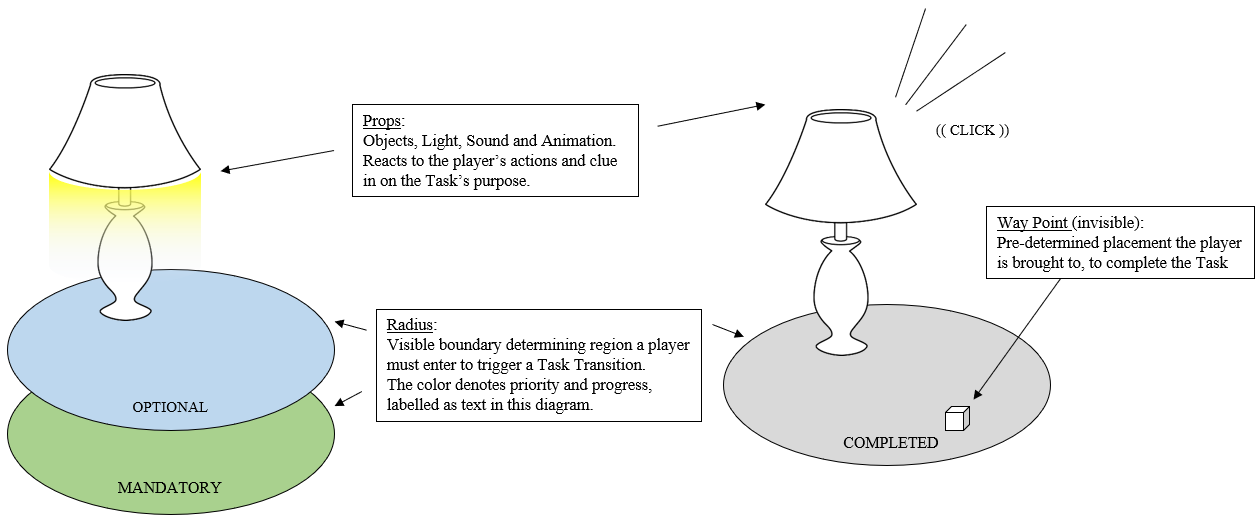
\includegraphics[width=0.95\paperwidth]{figures/InteractionSpaceDesign.png}
            \caption{\label{fig:FigureInteractionSpace}Overview of Interaction Space's Design Elements}               
    \end{figure}
    

\subsection{Player Character Design} \label{sec:develop_character}

    Given that the game was supposed to be a natural and immersive experience, no attention was desired to be brought to a character the user controls. Rather than creating one, the intent was to create an outward sense of belonging into the virtual world, as if the user could say “I am the character on-screen”. Implementing a person even just through aesthetic design could compromise that plan. This was the reason why the game was built with its first-person perspective, that would eliminate the need for any visible character traits on-screen or any latent thought of piloting something over those of self-control.\\
    However, merely showing nothing has one significant issue related to the novelty of the technology used. The Leap Motion is primarily used as an accessory apparatus to Virtual Reality experiences and games, and VR is itself a still uncommonly used technology, with many folks not having first hand experiences with it. The volunteers were predicted to not be completely aware of correct usage or limitations of the device unless if the game provided such feedback live as it occurs, and there isn’t enough time during a user trial to reach the level or proficiency required to innately recognize problems as they arise. A virtual representation of the player’s hand isn’t just a suggestion brought up by other applications of the Leap Motion device, but a requirement that must be present within the game, as then, the user is capable of discerning not just if they’re doing the correct gesture from the representation, but also if the application finds that they’re doing the correct gesture as well, or if small corrections will be required.\\
    Here, a decision is made that is at odds with the problem that caused the choice itself. What should the hand look like? There’re essentially only two possibilities: Either the hand looks realistically, but inevitably appears different from the user’s own real hand and a dissonance is established; or the hand is made to appear like an unambiguously digital approximation of a hand with simpler shapes. There were two at least two hand models provided by the Leap Motion’s library of assets that made either choice possible without much trouble. Given the two choices, no benefit is posed by the first option, and a lesser consistent experience among volunteers was predicted, not to mention the potential source for distraction provided by the more visually enticing.  There was a third option, giving the user a choice of hand model among a larger number, however, that could also pre-emptively give too much of an importance to the hand’s look, which is an undesirable outcome if avoidable. \\
    As such, during the game, the player can see a hand’s model built of simple gray and blue smooth shapes denoting fingers and joints, functioning as a proxy to the player’s own hand, and reacting to movement by performing the same gestures and staying at a similar depth and distance as the player’s own real hand would, mimicking a first person’s field of view with a raised hand.\\

    \begin{figure}[ht]
        \centering                                                
        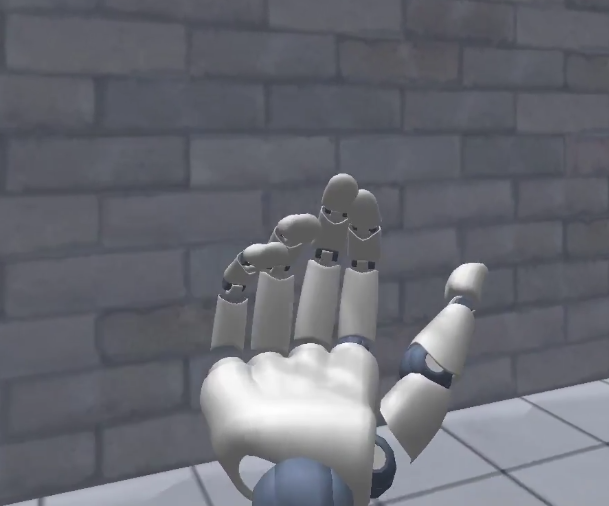
\includegraphics[width=0.3\paperwidth]{figures/HandIngame.png}
        \caption{\label{fig:FigureHand}Screen Capture of the in-game Hand Model}               
    \end{figure}

\subsection{Enviroment Design} \label{sec:develop_game_enviroment}

    The game occurs in a single virtual environment. Once it begins, there are no loading screens and any pauses happen only due to the game’s own interactive make up rather than to needing to load more assets. The only complex background processing required involves the classifier switching and even this should be a seamless and instant process. In other words, the game is small enough to be fully loaded at all times.
    Yet, it should also have been big enough that there isn’t a perception overload to the player with too many tasks and options present at a time. A large multiplicity of cues can confuse or frustrate the user. Given that there are 8 total tasks in the game separated in two groups of four, it was found appropriate to separate these into pairs of two tasks, one mandatory and one optional, and placed within four rooms. Additionally, to streamline the process of finding these tasks, the rooms were laid out in sequence through connecting corridors.\\
    
    \begin{figure}[ht]
        \centering
        \hspace*{-1cm}
        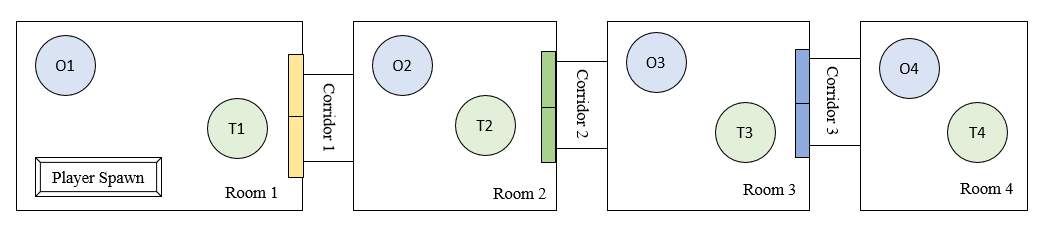
\includegraphics[width=0.8\paperwidth]{figures/RoomOverview.png}
        \caption{\label{fig:FigureRooms}Overview of the virtual enviroment's Room Design}
    \end{figure}

    One of the things that such a sequential line-up opens to the game is the chance of someone missing out on the presence of a task. This is undesirable, as detracting user choice from the completion of a task gives off less information about the task itself, than someone intentionally avoiding it or performing it and giving a bad grade. Opposed, to it, it does permit to observe one of the subtler factors of immersive experiences, assumingly, the user’s level of comfort and confidence with the controls, which are often overstated in self-assessments. Ultimately, the proposition of an intuitive cue for progress trumps over alternatives.\\
    Rooms are therefore separated by gates that do not open until the containing mandatory task is finished. Moreover, the transition between rooms is not just identified by the crossing of a gate, but also visually by the rooms themselves, as the looks of the floor, walls and ceilings changes drastically upon entering a corridor and matches with the following area. Also, to better attach the completion of a mandatory task with its correspondent gate, these gates were colored, and a key was integrated as part of the task’s completion.\\
    Other guiding elements are also present within rooms. Green arrows appear near gates, corridor entrances or on empty walls to help direct the user and reinforce that they’re heading the correct direction. Non-interactive plants are present on empty corner to fill the empty space and give the impression of a location of no interest to the game’s progress. Also, the empty play area with no object of interest is progressively funnelled in size, as the player is expected to make lesser mistakes in their movement as they progress and would find less of a reason to take large exploratory measures with the controls.\\ 
    This last point touches on the subject of room layout, which brings up the question of task placement. Of the two tasks in each room, the mandatory task is always placed closest to the exit gate and furthest to the entrance. The optional tasks however are progressively brought into the most direct path of the player. In order: O1 is on an indentation to the left of the room, O2 is off to the left but within the regular room boundaries, O3 is to the left of the path, but directly in front of the player from where they would come into the room, and finally, O4 is completely in the way of the player and they must sidestep it if they don’t want to compete the task. Additionally, O1 and O2 represent tasks that don’t lend themselves to having very much of an immediate urgency in nature, while O3 and O4 represent something that demands hurriedness from the user, and something that is just bothersome and has to be dealt with right away, thus justifying their progressive shift from staying away to getting in the way.\\
    
    \begin{figure}[ht]
        \centering
        \hspace*{-1cm}
        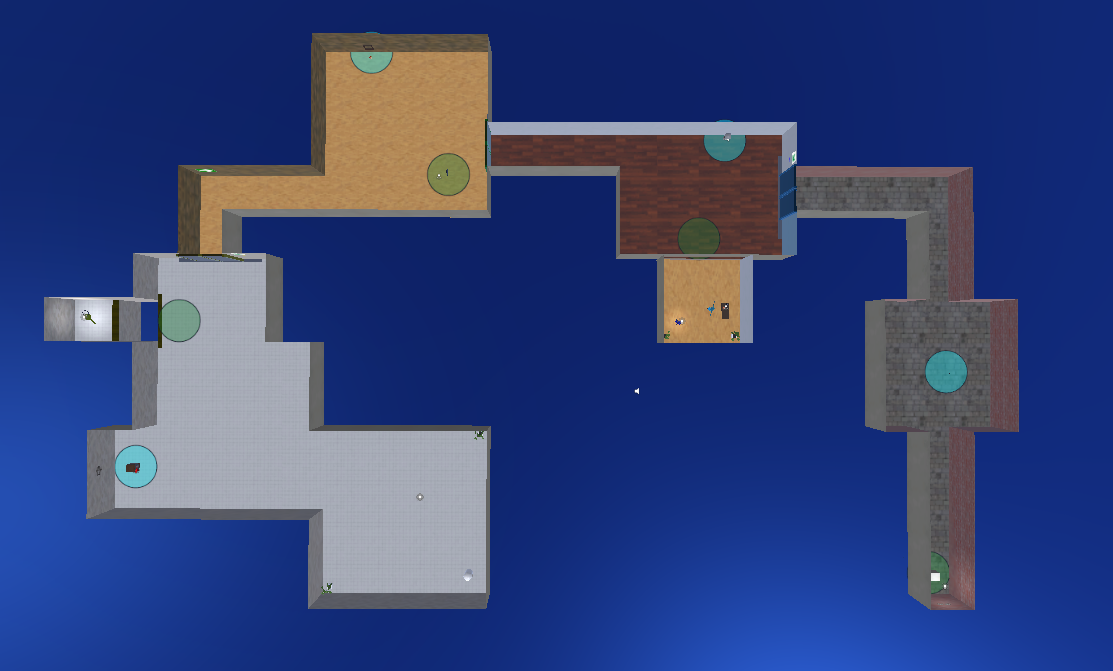
\includegraphics[width=0.8\paperwidth]{figures/Overhead.png}
        \caption{\label{fig:FigureGameOverhead}Overhead view of the game's virtual enviroment}
    \end{figure}

\subsection{Game Logic} \label{sec:develop_game_logic}
    For its implementation on Unity, the game has 4 core elements. These are the \emph{GameController}, \emph{CharacterController}, \emph{InteractionSpaceController} and \emph{CinematicHandler} scripts. Many other scripts were relevant to the game’s function, however, all of those had a small role within restrained contexts, and worked in a master, slave manner to one of these core scripts, such as, for example, the RadomFlight handler script, that made task O4’s insects move erratically, does not interact with any script besides the CinematicHandler and does so only on one moment in the game, during the closing transition of the O4 interaction space.\\
    The \emph{GameController} is tasked with initializing the game’s Shamanic Interface and defining state definitions that the game will require. It is also the game controller that will dispense a new classifier during task transitions. Thus, this Is an entry point for the Character Controller and the Interaction Space Controller during those times. It is also the GameController that defines the game’s culture, and it is here that I found the single difference between the game build presented to the Cultural and Non-Cultural groups. The Non-cultural group plays with an undefined Culture and thus the game uses the SI’s default gestures. Meanwhile, the Cultural group defines its culture as “PT” and those gestures get overridden by the pairs belonging to it. The code snippet corresponding to gesture efinition can be found on appendix \ref{ap1:InitCulturalLayer}. There’s a single Game Controller object in the game space and the other core scripts have a reference and access to it at any given moment.\\
    The Character Controller is a long script with definitions related to accepting input from the Leap Motion device (or Keyboard, for debugging purposes) to move the player’s camera around the virtual environment or to complete tasks. It’s here that the game checks if the classifier yields the correct gesture and if it’s also here that the game informs the rest of the system what gesture is currently being performed. It’s also where the game’s current valid options for control are changed, and where collision between a player and an interaction space’s region is handled. Ironically, the Character Controller is not statically aware of any command definition, merely matching what the classifier informs it, with the current Task. Its task completion code being agnostic to the definitions allows it to function if new definitions are set up. In summation, anything related to player input or to changing what a player can do has its entry point here.\\ 
    However, it’s the Interaction Space Controller that defines what those gestures are for each task, and if they’ve been performed for long enough to accrue to the task’s completion. While there is a single Character Controller there’s a different instance of the Interaction Space Controller attached to the corresponding game objects. Every interaction space object has its own script, with its own different internal settings correspondent to a different Task. Upon collision of the Player and an Interaction Script, the scripts belonging to each attach to each other, and a back process of communication ensues through the 3 Scripts. The Interaction Space controller informs the Character Controller of what Task is performed within the interaction space, and the Character Controller then requests the Game Controller To feed that task’s correspondent State into its Shamanic Interface. Finally, the Game Controller yields the resulting Classifier back to the Character Controller, and the Character Controller will from then on inform the Interaction Space every frame that a gesture was performed. State definition code snippets can be found in \ref{ap1:StateDefinitions}.\\
    This happens relatively instantaneously, albeit, there is some leeway to give the Shamanic Interface some time for returning the Classifier, as at the very first moment of the collision between player and Interaction Space, an initial task transition phase, called player repositioning, is executed. During these, the character controller actually removes control from the player for three seconds and forcefully moves them to an appropriate spot where they will perform the task’s gestures.\\
    And, finally, the Cinematic Handler, which synchs and performs visual and audible alterations to the environment during intermediate and final task transition phases. From moving and animating object, to dimming lights and turning off sounds, this provide the player with the feedback that a Task was completed by changing the task’s props in some manner. Only the Interaction Space Controller communicates with it, which means that granting player control after a Task’s completion must be done through it as a middleman between the Cinematic Handler and the Character Control Script.\\

    \begin{figure}[ht]
        \centering
        \hspace*{-1cm}
        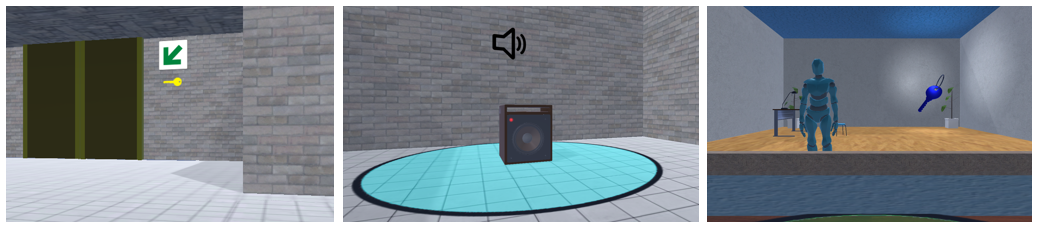
\includegraphics[width=0.8\paperwidth]{figures/IngameScreenshots.png}
        \caption{\label{fig:FigureScreenshots}Screenshots of the Game Enviroment}
    \end{figure}
\section{Survey Data} \label{sec:results_surveys}

\subsection{Usability Report} \label{sec:results_surveys_usability}
    Given that this game was built from scratch, there’s one important aspect that was not previously researched. A proper usability test was never performed on it thoroughly. Some aspects of the game that were verified rougher, such as movement, may have perhaps had a chance for improvement with time given towards taking user feedback and reworking of those trouble spots.\\
    So why is measuring usability important during the trials then? Because ease of use, learnability and repeatability are some of the most important indicators by which satisfaction is evaluated, and the majority of methodologies used in Human-Computer Interaction research to validate assumptions into concrete ideas are variations of usability tests. This present work itself is similar in nature to one method of testing usability, known as Split Testing, whereas two versions of an application are handed to different groups and variations in key metrics are determined. In sum, the measurement of usability is indissociable from any form of research involving user interaction.\\
    To perform this study on the system’s usability, we resorted to the System Usability Scale\cite{brooke1996sus}, the SUS. The SUS is an industry standard questionnaire consisting of ten elements to which users respond in a scale between strong disagreement and strong agreement. These questions were adapted to the game into the post-game survey and rearranged, however the function of the SUS’s scoring is intact. Table \ref{tab:Table_SUS} shows these scores.\\
    \begin{table}[ht]
    \begin{tabular}{ll}
    \hline
    \multicolumn{1}{|l|}{Cultural}     & \multicolumn{1}{l|}{SUS Score} \\ \hline
    \multicolumn{1}{|l|}{V1}           & \multicolumn{1}{l|}{87.5}      \\ \hline
    \multicolumn{1}{|l|}{V3}           & \multicolumn{1}{l|}{80}        \\ \hline
    \multicolumn{1}{|l|}{V5}           & \multicolumn{1}{l|}{90}        \\ \hline
    \multicolumn{1}{|l|}{V6}           & \multicolumn{1}{l|}{85}        \\ \hline
    \multicolumn{1}{|l|}{V9}           & \multicolumn{1}{l|}{90}        \\ \hline
    \multicolumn{1}{|l|}{V11}          & \multicolumn{1}{l|}{87.5}      \\ \hline
    \multicolumn{1}{|l|}{V13}          & \multicolumn{1}{l|}{85}        \\ \hline
    \multicolumn{1}{|l|}{V15}          & \multicolumn{1}{l|}{85}        \\ \hline
    \multicolumn{1}{|l|}{V17}          & \multicolumn{1}{l|}{92.5}      \\ \hline
                                       &                                \\ \hline
    \multicolumn{1}{|l|}{Non-Cultural} & \multicolumn{1}{l|}{SUS Score} \\ \hline
    \multicolumn{1}{|l|}{V2}           & \multicolumn{1}{l|}{65}        \\ \hline
    \multicolumn{1}{|l|}{V4}           & \multicolumn{1}{l|}{77.5}      \\ \hline
    \multicolumn{1}{|l|}{V7}           & \multicolumn{1}{l|}{72.5}      \\ \hline
    \multicolumn{1}{|l|}{V8}           & \multicolumn{1}{l|}{80}        \\ \hline
    \multicolumn{1}{|l|}{V10}          & \multicolumn{1}{l|}{80}        \\ \hline
    \multicolumn{1}{|l|}{V12}          & \multicolumn{1}{l|}{87.5}      \\ \hline
    \multicolumn{1}{|l|}{V14}          & \multicolumn{1}{l|}{65}        \\ \hline
    \multicolumn{1}{|l|}{V16}          & \multicolumn{1}{l|}{75}        \\ \hline
    \end{tabular}
        \caption{\label{tab:Table_SUS}System Usability Scale scores determined by the users of the Cultural and Non-Cultural Groups}
    \end{table}
    
    Between the two groups it’s apparent that the Non-cultural group had a lesser impression related to the game’s usability. While this was a unanimous complaint, the lowest SUS scores were also coming from the volunteers who most felt the need to verbalize their discontent with the game’s movement. The SUS score ranges from 0 to 100, however these are not percentages spread over a uniform distribution. There’s no single guideline by which all SUS scores are interpreted, but what is usually accepted as a good parameter, is that a desirable threshold to surpass is a SUS score of 68, which represents an approximated average of most SUS questionnaires, or alternatively a score of 80, which is associated with high task completion\cite{sauro2011practical}, although these values may vary depending on the researcher heading the questionnaire, sample sizes and sample selection. There are more benchmarks and percentile breakdowns, but in broad terms, it’s valid to state that the Cultural Group’s is set above the Non-Cultural Group by at least a ranking in terms of its usability, and thus, the choice of gestures has provided a benefit to the Cultural Group.\\

\subsection{Confidence and Culturally-Driven Misplaced Confidence} \label{sec:results_surveys_confidence}
    After the games were completed, the participants were asked about each of the individual tasks they performed on a number of aspects. Aspects such as how they felt about solving them, if the gesture felt natural, among others. One of which, exclusive to the second trial, was their confidence in remembering the task's gestures, and, conversely, if they had trouble remembering it. A few more questions not related to the tasks directly allowed to further get a feel for their personal evaluation on the matter.\\
    From these, it was possible to rate each user's global confidence in solving the game's tasks on a scale ranging from 0 to 30. However, this is not a metric that's very useful on its own. Beyond the fact that a user's confidence may be related to personal facets and quirk's, we're also not looking into if the game on its own inspires confidence, but rather if the cultural emblems within a fitting context are a major differentiator for the users otherwise experiencing the same game. This means that merely comparing the Cultural and Non-Cultural Group's Confidence Score wouldn't be enough.\\
    It was considered important to go back to the game performance assessment and attempt to categorize the sources of confidence in separate ways. The confidence score would remain a global perspective of the user's evaluation, but a sub-score of it would list out how much of that confidence was misplaced and borne of a user performing the wrong action and still clearing the task. Thus, we may create two scores, a participant's Confidence score, and a Misplaced Confidence score. But this approach is still insufficient, as the cultural component is missing. It's by taking in account the types of Gestural Mistakes observed earlier \ref{sec:results_game_performance} that this misplaced confidence becomes relevant.\\
    Ideally for the thesis' hypotheses, for each user that committed a mistake in the game yet claimed confidence that they solved it correctly, they would have done so because they misremembered a well-fitting cultural emblem in place of their actual mistaken gesture. As such, another score is required to be broken down from confidence, that of the Culturally-Driven Misplaced Confidence.\\
    
    \begin{table}[ht]
    \begin{tabular}{llll}
    \cline{2-4}
    \multicolumn{1}{l|}{}     & \multicolumn{1}{l|}{Total} & \multicolumn{1}{l|}{Misplaced} & \multicolumn{1}{l|}{Cultural} \\ \hline
    \multicolumn{1}{|l|}{V1}  & \multicolumn{1}{l|}{26}    & \multicolumn{1}{l|}{0}         & \multicolumn{1}{l|}{0}        \\ \hline
    \multicolumn{1}{|l|}{V3}  & \multicolumn{1}{l|}{27}    & \multicolumn{1}{l|}{0}         & \multicolumn{1}{l|}{0}        \\ \hline
    \multicolumn{1}{|l|}{V6}  & \multicolumn{1}{l|}{24}    & \multicolumn{1}{l|}{0}         & \multicolumn{1}{l|}{0}        \\ \hline
    \multicolumn{1}{|l|}{V9}  & \multicolumn{1}{l|}{23}    & \multicolumn{1}{l|}{0}         & \multicolumn{1}{l|}{0}        \\ \hline
    \multicolumn{1}{|l|}{V11} & \multicolumn{1}{l|}{19}    & \multicolumn{1}{l|}{0}         & \multicolumn{1}{l|}{0}        \\ \hline
    \multicolumn{1}{|l|}{V13} & \multicolumn{1}{l|}{30}    & \multicolumn{1}{l|}{0}         & \multicolumn{1}{l|}{0}        \\ \hline
    \multicolumn{1}{|l|}{V15} & \multicolumn{1}{l|}{26}    & \multicolumn{1}{l|}{0}         & \multicolumn{1}{l|}{0}        \\ \hline
    \multicolumn{1}{|l|}{V17} & \multicolumn{1}{l|}{28}    & \multicolumn{1}{l|}{0}         & \multicolumn{1}{l|}{0}        \\ \hline
                              &                            &                                &                               \\ \cline{2-4} 
    \multicolumn{1}{l|}{}     & \multicolumn{1}{l|}{Total} & \multicolumn{1}{l|}{Misplaced} & \multicolumn{1}{l|}{Cultural} \\ \hline
    \multicolumn{1}{|l|}{V2}  & \multicolumn{1}{l|}{21}    & \multicolumn{1}{l|}{9}         & \multicolumn{1}{l|}{8}        \\ \hline
    \multicolumn{1}{|l|}{V4}  & \multicolumn{1}{l|}{22}    & \multicolumn{1}{l|}{12}        & \multicolumn{1}{l|}{8}        \\ \hline
    \multicolumn{1}{|l|}{V7}  & \multicolumn{1}{l|}{20}    & \multicolumn{1}{l|}{10}        & \multicolumn{1}{l|}{10}       \\ \hline
    \multicolumn{1}{|l|}{V8}  & \multicolumn{1}{l|}{30}    & \multicolumn{1}{l|}{0}         & \multicolumn{1}{l|}{0}        \\ \hline
    \multicolumn{1}{|l|}{V10} & \multicolumn{1}{l|}{24}    & \multicolumn{1}{l|}{12}        & \multicolumn{1}{l|}{10}       \\ \hline
    \multicolumn{1}{|l|}{V12} & \multicolumn{1}{l|}{25}    & \multicolumn{1}{l|}{20}        & \multicolumn{1}{l|}{20}       \\ \hline
    \multicolumn{1}{|l|}{V14} & \multicolumn{1}{l|}{23}    & \multicolumn{1}{l|}{8}         & \multicolumn{1}{l|}{4}        \\ \hline
    \multicolumn{1}{|l|}{V16} & \multicolumn{1}{l|}{22}    & \multicolumn{1}{l|}{3}         & \multicolumn{1}{l|}{3}        \\ \hline
    \end{tabular}
        \caption{\label{tab:Table_Confidence}Confidence Scores showcased by Cultural and Non-Cultural groups during the second trial}
    \end{table}
    
    Since the Cultural group made no definite gestural mistakes, their misplaced scores can only be zero, and their culturally-driven misplacement, while possible in practice, would require issues with the task design itself, which was precisely the reason why two were eliminated from the evaluation. One way or another, while confidence is an important metric for the global experience assessment, the whole Cultural group is not really insightful for this current approach. However, as for the Non-Cultural Group, a lot of the score is valid. Since nearly the complete majority of the gestural mistakes were Emblematic Substitutions, it's no surprise that a lot of the confidence the users had misplaced was sourced to their cultural expectations. Manifestly, 85\% of all of the misplaced user confidence score was due to the Non-Cultural trial intentionally breaking their natural conventions. Given an application with more direct forms of feedback where it comes to user failure, this data favors the gesture set employed by the Cultural group enormously.
    
\subsection{Global Experience and Immersiveness Indicators} \label{sec:results_surveys_immersiveness}
    To properly evaluate the global experience of the game in both game’s post-tests, a choice was factors considered relevant would be required. Giving the volunteers more freedom in reporting their relevant determinants was considered and would be valuable for the general evaluation. Such as the PANAS scale, for a tallying of subjective mood. However, the need for a comparative evaluation between test groups dictated that the post-test surveys would have to be more focused at a pre-determined set of elements between the two user groups, that covered more aspects than affectivity.\\
    With other questions in the post-test, the game, the Content component in the UX triad, was already looked at in several manners. A proper UX questionnaire ought to look into the other two elements of interaction: The Person, their experience, their anticipations, their characteristics, their relationships; and the Form, the technology by which the game is delivered, the extra content not part of the game’s primary progression. The latter is interesting mostly in aspects that may have affected the former, as people’s focus and attention is performed in a generally scattered yet not truly expectable manner. What some find amusing, distracting and correctly perceive, others may fail to because of form factors. That is to say, most of the questions in the post-game were majorily introspective, framing questions from the perspective of what the participants felt and responded to, rather than questioning about the game (E.g. "I have enjoyed myself" instead of "The game was enjoyful").\\
    The following were the indicators chosen: Emotional Impact; Internal Expectations; Self-Consciousness; External Expectations and Sharing; Recall and Recognition; Enjoyment and Repeatability; Subjective Sense of Comfort; Technological and Methodological Impact; Symbolic Feedback and Sense Making. Some indicators were also ascertained in other works but didn’t feel like they fit well with the current, such as Monetary Value, the willingness to pay money for similar experiences; or Reputation, which did not make sense given the fact the technology was almost entirely unknown to the participants prior. These were asked to the volunteers through questionnaire, and the answers were weighed to a scale ranging from 0 to 50, the higher the better. Table \ref{tab:Table_Final} shows the scores for each indicator, for each of the Cultural and Non-Cultural Groups.\\
    
    \begin{table}[ht]
    \begin{tabular}{llll}
    \cline{1-2}
    \multicolumn{1}{|l|}{Cultural Group}                          & \multicolumn{1}{l|}{score} &                       &                                     \\ \cline{1-2} \cline{4-4} 
    \multicolumn{1}{|l|}{Emotional Impact}                        & \multicolumn{1}{l|}{43.75} & \multicolumn{1}{l|}{} & \multicolumn{1}{l|}{Total}          \\ \cline{1-2} \cline{4-4} 
    \multicolumn{1}{|l|}{Internal Expectations}                   & \multicolumn{1}{l|}{37.50} & \multicolumn{1}{l|}{} & \multicolumn{1}{l|}{382.60}         \\ \cline{1-2} \cline{4-4} 
    \multicolumn{1}{|l|}{Self-Consciousness}                      & \multicolumn{1}{l|}{47.92} &                       &                                     \\ \cline{1-2} \cline{4-4} 
    \multicolumn{1}{|l|}{External Expectations and Sharing}       & \multicolumn{1}{l|}{43.75} & \multicolumn{1}{l|}{} & \multicolumn{1}{l|}{Mean}           \\ \cline{1-2} \cline{4-4} 
    \multicolumn{1}{|l|}{Recall and Recognition}                  & \multicolumn{1}{l|}{43.75} & \multicolumn{1}{l|}{} & \multicolumn{1}{l|}{42.51}          \\ \cline{1-2} \cline{4-4} 
    \multicolumn{1}{|l|}{Enjoyment and Repeatability}             & \multicolumn{1}{l|}{43.75} &                       &                                     \\ \cline{1-2} \cline{4-4} 
    \multicolumn{1}{|l|}{Subjective Sense of Comfort}             & \multicolumn{1}{l|}{43.75} & \multicolumn{1}{l|}{} & \multicolumn{1}{l|}{Std  Deviation} \\ \cline{1-2} \cline{4-4} 
    \multicolumn{1}{|l|}{Technological and Methodological Impact} & \multicolumn{1}{l|}{40.63} & \multicolumn{1}{l|}{} & \multicolumn{1}{l|}{3.31}           \\ \cline{1-2} \cline{4-4} 
    \multicolumn{1}{|l|}{Symbolic Feedback and Sense Making}      & \multicolumn{1}{l|}{37.81} &                       &                                     \\ \cline{1-2}
                                                                  &                            &                       &                                     \\ \cline{1-2}
    \multicolumn{1}{|l|}{Non-Cultural Group}                      & \multicolumn{1}{l|}{score} &                       &                                     \\ \cline{1-2} \cline{4-4} 
    \multicolumn{1}{|l|}{Emotional Impact}                        & \multicolumn{1}{l|}{50.00} & \multicolumn{1}{l|}{} & \multicolumn{1}{l|}{Total}          \\ \cline{1-2} \cline{4-4} 
    \multicolumn{1}{|l|}{Internal Expectations}                   & \multicolumn{1}{l|}{28.13} & \multicolumn{1}{l|}{} & \multicolumn{1}{l|}{342.59}         \\ \cline{1-2} \cline{4-4} 
    \multicolumn{1}{|l|}{Self-Consciousness}                      & \multicolumn{1}{l|}{45.83} &                       &                                     \\ \cline{1-2} \cline{4-4} 
    \multicolumn{1}{|l|}{External Expectations and Sharing}       & \multicolumn{1}{l|}{43.75} & \multicolumn{1}{l|}{} & \multicolumn{1}{l|}{Mean}           \\ \cline{1-2} \cline{4-4} 
    \multicolumn{1}{|l|}{Recall and Recognition}                  & \multicolumn{1}{l|}{24.31} & \multicolumn{1}{l|}{} & \multicolumn{1}{l|}{38.07}          \\ \cline{1-2} \cline{4-4} 
    \multicolumn{1}{|l|}{Enjoyment and Repeatability}             & \multicolumn{1}{l|}{46.88} &                       &                                     \\ \cline{1-2} \cline{4-4} 
    \multicolumn{1}{|l|}{Subjective Sense of Comfort}             & \multicolumn{1}{l|}{47.92} & \multicolumn{1}{l|}{} & \multicolumn{1}{l|}{Std  Deviation} \\ \cline{1-2} \cline{4-4} 
    \multicolumn{1}{|l|}{Technological and Methodological Impact} & \multicolumn{1}{l|}{34.38} & \multicolumn{1}{l|}{} & \multicolumn{1}{l|}{11.12}          \\ \cline{1-2} \cline{4-4} 
    \multicolumn{1}{|l|}{Symbolic Feedback and Sense Making}      & \multicolumn{1}{l|}{21.41} &                       &                                     \\ \cline{1-2}
    \end{tabular}
        \caption{\label{tab:Table_Final}Immersiveness Factors and Scores between the Two Groups}
    \end{table}
    There was a tendency by the users to give consistent responses sticking mostly to full or light agreement. This is why, despite having different number of dimensions (questions), 4 of the parameters in the Cultural Group had the same score in a pattern. The Non-CulturalGroup scores lower than the Cultural overall, and it would appear that three of the factor are very much lower than the Cultural's. But it's not credible enough that this is a significant difference without data analyticals.\\
    Performing a double ailed two-sample t-test, we can attempt to validate an hypothesis by bidding to prove an opposing one. By seeking to credit that the samples have similar characteristics, we could perhaps find suggesting evidence at a given level of significance that the games had different impacts on the players. However, at a significance level of 0.05, we already find no convincing enough evidence (t= 1.149818588, tc= 2.262157163) that the two samples differ significantly. And given that at, at p-value 0.05, there's at least 23\% (and typically close to 50\%) chance of incorrectly suggesting the alternate hypothesis, this proves to not be a valid vector by which difference between the two groups can be established. In summation, the immersiveness indicators were inconclusive.\\
    
\subsection{Loose Observations} \label{sec:results_surveys_disjointed}
    Both cultural and non-cultural groups were requested to name the most memorable part of the game. Out of 4 exceptions, both parties named the same element. Those exceptions include 2 users speaking of their frustration with movement, and 2 speaking of the moment of victory. All remaining 13 users singled out the blue animated humanoid NPC due to the richness of its responsiveness and interaction. Also, as noted earlier, this NPC reacted by performing its own gestures, two of which were done in a similar fashion to the Cultural Group's (Waving and Pointing), which may have influenced the Non-Cultural Group's memory of the experience.\\
    On the second part of the second trial's post-test, after the being questioned about the tasks, the volunteers were asked about substitutions to the gesture set, while also being reminded of what the actual gesture set was. Out of 19 (17 from the Non-Cultural Group) suggestions, only 1 did not involve a cultural gesture, and only an additional 2 didn't involve emblematic gestures. Non-Cultural Group participants were fixated on gestures that ended up belonging to the Cultural gesture set.\\
\section{Conclusions} \label{sec:results_Conclusions}
    This work reported on a number of findings of two sets of user trials to assess impacts of measures on the quality of several aspects of UX, by means of, primarily, a comparative test. The purpose of these findings was to validate three initial propositions offered before the start of planning and development of the work. Of these three items, two have been found conclusive, while another did not come to be, and should require a different approach with a number of alterations.\\
    \begin{itemize}
        \item \textbf{Focusing on user culture contributes to the learning rate and capacity of commands; and to the Retention and Memorization of commands and concepts}\\
            On several passages throughout section \ref{sec:results_game} it is referenced that the majority of the Cultural Group performed exceptionally well during both game trials. Very few errors and failures were registered on the first trial, and coming into the second, the group even flourishingly carried on to manifest growth and improvement over the earlier trial. This in contrast to the Non-Cultral Group, which had trouble assimilating and present the corect commands, and in due, saw a worsening development of performance after the two week delay. Aspects of confidence, anticipation and memory were also among the descriptors looked into that illustrated a reduced positive impact on the Non-Cultural Group independent from the performance evaluation. Coming back to said evaluation, it becomes palpable that the Non-Cultural Group didn't just become unsucessful and fell short based on the choice of gesture set given, but moreover, also due to the group seeking out the what was the approapriate gesture for the game's context, which coincided with the Cultural Group's gesture set. This persistence even poisons the Non-Cultural recolection, making them feel certainty and assurance which has been ultimately misplaced, indicating that the Cultural gesture set was not just prefered among the two, but potentially, the most natural choice for the situation.
            
        \item \textbf{Focusing on user culture contributes to the satisfaction and immersion of the experience}\\
            Two measures were performed primarily towards this during the work. The usability report was insightful, proving that there was a highly significant difference \emph{(p=0.0031)} in the game between the Groups in terms of the system's capabilities to deliver a satisfying entertaining experiece. But one set of measures wasn't enough, and one another more comprehensive invstigation into immersiveness and satisfaction did not produce further corroboration. It's not improbable that this benefit is still factual, and it's possible to suppose from certain observations and moments in the game, particularly involving task T3, that this could be better observed with greater quality of superficial design.
    \end{itemize}

\section{Closing Thoughts and Future Work} \label{sec:results_End}
    With this work, we have consolidated the idea that cultural emblems are natural and can symbolically benefit users to organically with the initial barrier of entry to using a NUI. By testing a game built around the context of solving gestures, users are prone to resorting to these emblems they know of, and are moreover, it makes it accessible if recall the commands if necessary. But more needs to be tested and done so more rigorously.\\
    Satisfaction and Immersion have not been properly justified, as noted above, but there's more to investigate. The current findings all aim towards benefits involving the initial usage hurdle of an application, it tests out easy to perform tasks, even if these involve multiple steps. While there was a plan to look into separating tasks into easy and hard tasks, this never quite came into fruition. The justification for Optional and Mandatory tasks was such that, besides the very first optional task, these would all involve larger struggle towards resolution. Some ideas for what this difficulty would ensue were written down, such involving gesturing towards objects with motions that would make sense only if aiming to address an intelligent receiver. However, neither was any solution really acceptable, the approach itself didn't seem very lenient towards a good analysis. Still, it would be deemed really useful to make one potential analysis of the upper parameters of complexity. To test out if adaptable Cultural Gestures do provide a benefit to Depth of Interaction. While learning and memory as advantages may be upheld right now, what degree of richness the interaction achieves is not.\\
    Another aspect of the application was unsatisfactory. Player Movement was too contrived by a composite issue of the transition between movement gestures, the Leap Motion having certain faults in perceiving movement with the palm pointed upwards, and with the game itself not smoothing out the rotation speed of turning very gracefully. However, in hindsight, it's very possible that movement in general may have not been a very insightful act to observe in the first place. Additionally, movement is not something that is customarily performed in a natural fashion even in recent immersive systems, such as virtual reality experiences, which relies heavily on either unconventional player teleportation to achieve large distances or using a controller’s analog stick for advancing through the world, both approaches which clearly unfit for a fully Natural Interface.\\
    \\
    Thus we suggest the following directives towards a development of future system: Improve the Classifier, bring a new and better approach to the recognition of hand gestures such as machine learning approaches; Create a Virtual Reality environment to test the participants in a more immersive setting, or alternatively, create an Amplified Reality game such that the environment is virtually super-imposed over the real world setting; Focus primarily on the Task setup, remove long duration requirements between each focal point of the observation, such as movement; Make a good definition of task failure and give players a fixed number of attempts or time to complete them, make sure to employ proper feedback within the application on both aspects; Create a difficulty curve, make it so some of the tasks are clearly devised as more difficult than others; Test multiple cultural settings, find valid gesture sets for more than one culture and verify that the benefits permeate all of these over a non-cultural control group.\\
    

%%----------------------------------------
%% Final materials
%%----------------------------------------

%% Bibliography
%% Comment the next command if BibTeX file not used
%% bibliography is in ``myrefs.bib''
\bibliographystyle{unsrt}
\PrintBib{post-document/references}

%% Appendix
%% comment next 2 commands if numbered appendices are not used
\appendix
\chapter{Code Snippets} \label{ap1:CodeSnippets}

\section{Cultural Definition of Gestures within Game Controller as part of the Cultural Layer's Initialization} \label{ap1:InitCulturalLayer}

\begin{lstlisting}
public static void InitCulturalLayer() {
	//Common Gestures
	culturalLayer.AddDefaultGesture("NOTHING", "OPEN_HAND");
	culturalLayer.AddDefaultGesture("CANCEL", "WAVE");
	culturalLayer.AddDefaultGesture("NO", "THUMBS_DOWN");
	culturalLayer.AddDefaultGesture("YES", "THUMBS_UP");
	culturalLayer.AddDefaultGesture("THUMBS_DOWN", "THUMBS_DOWN");
	culturalLayer.AddDefaultGesture("THUMBS_UP", "THUMBS_UP");
	culturalLayer.AddDefaultGesture("FRONT", "POINT_FRONT");
	culturalLayer.AddDefaultGesture("BACK", "POINT_BACK");
	culturalLayer.AddDefaultGesture("RIGHT", "POINT_RIGHT");
	culturalLayer.AddDefaultGesture("LEFT", "POINT_LEFT");

	//List of default gestures here.
	culturalLayer.AddDefaultGesture("QUIET", "THUMBS_DOWN");
	culturalLayer.AddDefaultGesture("COME_HERE", "WAVE");
	culturalLayer.AddDefaultGesture("PHOTO_FRAME", "OK_RING");
	culturalLayer.AddDefaultGesture("IMPATIENT", "STOP");
	culturalLayer.AddDefaultGesture("PHONE", "LIFT_POINTER_FINGER");
	culturalLayer.AddDefaultGesture("ATTENTION", "THUMBS_UP");
	culturalLayer.AddDefaultGesture("POINT_AT", "POINT_FINGERGUN");
	culturalLayer.AddDefaultGesture("GO_AWAY", "WAVE");
	culturalLayer.AddDefaultGesture("CELEBRATE", "THUMBS_UP");

	//List cultural gestures here
	culturalLayer.AddCultureGesture("QUIET", "PT", "QUIET_NEW");
	culturalLayer.AddCultureGesture("COME_HERE", "PT", "COME_HERE");
	culturalLayer.AddCultureGesture("PHOTO_FRAME", "PT", "PHOTO_FRAME");
	culturalLayer.AddCultureGesture("IMPATIENT", "PT", "IMPATIENT");
	culturalLayer.AddCultureGesture("PHONE", "PT", "SHAKA_DOWN");
	culturalLayer.AddCultureGesture("ATTENTION", "PT", "ATTENTION");
	culturalLayer.AddCultureGesture("WAVE", "PT", "WAVE");
	culturalLayer.AddCultureGesture("POINT_AT", "PT", "POINT_AT");
	culturalLayer.AddCultureGesture("GO_AWAY", "PT", "SHOO");
	culturalLayer.AddCultureGesture("CELEBRATE", "PT", "FIST_PUMP");
}
\end{lstlisting}

\section{State Definitions within the Game Controller to be sent to the Cultural Layer by demand of the Character Controller} \label{ap1:StateDefinitions}

\begin{lstlisting}
public static State GoAwayState() {
	State state = new State("Shoo Away State");
	state.AddGesture("NOTHING");
	state.AddGesture("GO_AWAY");
	return state;
}

public static State VictoryState() {
	State state = new State("Victory State");
	state.AddGesture("NOTHING");
	state.AddGesture("CELEBRATE");
	return state;
}

public static State PhotoState() {
	State state = new State("Photo State");
	state.AddGesture("NOTHING");
	state.AddGesture("PHOTO_FRAME");
	return state;
}
\end{lstlisting}

%% Index
%% Uncomment next command if index is required
%% don't forget to run ``makeindex pdis-en'' command
%\PrintIndex

\end{document}
